%=======================================================================
% riscv-spec.tex
%-----------------------------------------------------------------------

\documentclass[twoside,11pt]{book}

% Fix copy/pasting of ligatures in Acrobat
\input{glyphtounicode.tex}
\pdfgentounicode=1 %

% Package includes

\usepackage[utf8]{inputenc}
\usepackage[T1]{fontenc}

\usepackage{graphicx}
\usepackage{geometry}
\usepackage{array}
\usepackage{colortbl}
\usepackage[svgnames]{xcolor}

\usepackage[colorlinks,citecolor=Navy,linkcolor=Navy]{hyperref}
\usepackage{placeins}
\usepackage{longtable}
\usepackage{multirow}
\usepackage{float}
\usepackage{listings}
\usepackage{comment}
\usepackage{enumitem}
\usepackage{verbatimbox}
\usepackage{amsmath}

\usepackage[olditem,oldenum]{paralist}

% Setup margins

\setlength{\topmargin}{-0.5in}
\setlength{\textheight}{9in}
\setlength{\oddsidemargin}{0in}
\setlength{\evensidemargin}{0in}
\setlength{\textwidth}{6.5in}

% Useful macros

\newcommand{\note}[1]{{\bf [ NOTE: #1 ]}}
\newcommand{\fixme}[1]{{\bf [ FIXME: #1 ]}}
% \newcommand{\todo}[1]{\marginpar{\footnotesize #1}}

\usepackage[%
  colorinlistoftodos,
  prependcaption
]{todonotes}

\ifdefined\isdraft
  \newcommand{\TodoSide}[1]{\todo[color=red!20]{\textbf{To do}: #1}}
  \newcommand{\NoteSide}[1]{\todo[color=green!20]{\textbf{Note}: #1}}
  \newcommand{\Todo}[1]{\todo[inline, color=red!20]{\textbf{To do}: #1}}
  \newcommand{\Note}[1]{\todo[inline, color=green!20]{\textbf{Note}: #1}}
\else
  \newcommand{\TodoSide}[1]{}
  \newcommand{\NoteSide}[1]{}
  \newcommand{\Todo}[1]{}
  \newcommand{\Note}[1]{}
\fi


\newcommand{\wunits}[2]{\mbox{#1\,#2}}
\newcommand{\um}{\mbox{$\mu$m}}
\newcommand{\xum}[1]{\wunits{#1}{\um}}
\newcommand{\by}[2]{\mbox{#1$\times$#2}}
\newcommand{\byby}[3]{\mbox{#1$\times$#2$\times$#3}}

\newlength\savedwidth
\newcommand\whline[1]{%
  \noalign{%
    \global\savedwidth\arrayrulewidth\global\arrayrulewidth 1.5pt%
  }%
  \cline{#1}%
  \noalign{\vskip\arrayrulewidth}%
  \noalign{\global\arrayrulewidth\savedwidth}%
}

% Custom list environments

\newlist{tightlist}{itemize}{1}
\setlist[tightlist]{label=\textbullet,nosep}

\newenvironment{titledtightlist}[1]
{\noindent
 ~~\textbf{#1}
 \begin{tightlist}}
{\end{tightlist}}

\newenvironment{commentary}
{	\vspace{-1.5mm}
	\list{}{
		\topsep		0mm
		\partopsep	0mm
		\listparindent	1.5em
		\itemindent	\listparindent
		\rightmargin	\leftmargin
		\parsep		0mm
	}
	\item
	\small\em
	\noindent\nopagebreak\rule{\linewidth}{1pt}\par
	\noindent\ignorespaces
}
{\endlist}

%\newenvironment{discussion}
%{	\vspace{-1.5mm}
%	\list{}{
%		\topsep		0mm
%		\partopsep	0mm
%		\listparindent	1.5em
%		\itemindent	\listparindent
%		\rightmargin	\leftmargin
%		\parsep		0mm
%	}
%	\item
%	\small\em
%	\noindent\nopagebreak\rule{\linewidth}{1pt}\par
%	\noindent\textbf{Discussion:}
%}
%{\endlist}

% Other commands and parameters

\pagestyle{myheadings}
\setlength{\parindent}{0in}
\setlength{\parskip}{10pt}
\sloppy
\raggedbottom
\clubpenalty=10000
\widowpenalty=10000

% Commands for register format figures.

% New column types to use in tabular environment for instruction formats.
% Allocate 0.18in per bit.
\newcolumntype{I}{>{\centering\arraybackslash}p{0.18in}}
% Two-bit centered column.
\newcolumntype{W}{>{\centering\arraybackslash}p{0.36in}}
% Three-bit centered column.
\newcolumntype{F}{>{\centering\arraybackslash}p{0.54in}}
% Four-bit centered column.
\newcolumntype{Y}{>{\centering\arraybackslash}p{0.72in}}
% Five-bit centered column.
\newcolumntype{R}{>{\centering\arraybackslash}p{0.9in}}
% Six-bit centered column.
\newcolumntype{S}{>{\centering\arraybackslash}p{1.08in}}
% Seven-bit centered column.
\newcolumntype{O}{>{\centering\arraybackslash}p{1.26in}}
% Eight-bit centered column.
\newcolumntype{E}{>{\centering\arraybackslash}p{1.44in}}
% Ten-bit centered column.
\newcolumntype{T}{>{\centering\arraybackslash}p{1.8in}}
% Twelve-bit centered column.
\newcolumntype{M}{>{\centering\arraybackslash}p{2.2in}}
% Sixteen-bit centered column.
\newcolumntype{K}{>{\centering\arraybackslash}p{2.88in}}
% Twenty-bit centered column.
\newcolumntype{U}{>{\centering\arraybackslash}p{3.6in}}
% Twenty-bit centered column.
\newcolumntype{L}{>{\centering\arraybackslash}p{3.6in}}
% Twenty-five-bit centered column.
\newcolumntype{J}{>{\centering\arraybackslash}p{4.5in}}

\newcolumntype{t}{>{\ttfamily}l}

\newcommand{\instbit}[1]{\mbox{\scriptsize #1}}
\newcommand{\instbitrange}[2]{~\instbit{#1} \hfill \instbit{#2}~}
\newcommand{\reglabel}[1]{\hfill {\tt #1}\hfill\ }

\newcommand{\wiri}{\textbf{WIRI}}
\newcommand{\wpri}{\textbf{WPRI}}
\newcommand{\wlrl}{\textbf{WLRL}}
\newcommand{\warl}{\textbf{WARL}}

\newcommand{\implementationdefined}{\textsc{implementation defined}}

\newcommand{\unspecified}{\textsc{unspecified}}

\graphicspath{ {figures/} }


\newcommand{\specrev}{\mbox{1.1.2}}
\newcommand{\specmonthyear}{\mbox{November 2022}}

\begin{document}

\title{\vspace{-0.7in}\Large {\bf The RISC-V Xvpfloat Instruction Set Extension Manual} \\
  \large {\bf Volume I: Unprivileged ISA} \\
  Document Version \specrev
  \vspace{-0.1in}}

\author{Editors: Eric Guthmuller$^{1}$ \\
  $^{1}$CEA List \\
  {\tt eric.guthmuller@cea.fr} \\
  \today
}
\date{} 
\maketitle

Contributors to all versions of the spec in
alphabetical order :
Riccardo Alidori,
Andrea Bocco,
Yves Durand,
Jérôme Fereyre,
Cesar Fuguet Tortolero,
Eric Guthmuller.

This document is propriety of CEA.



\markboth{{\em CEA Confidential} - Volume I: RISC-V Xvpfloat Unprivileged ISA V\specrev}
{{\em CEA Confidential} - Volume I: RISC-V Xvpfloat Unprivileged ISA V\specrev}
\thispagestyle{empty}

\frontmatter

\chapter{Preface}

This document describes the RISC-V Xvpfloat extension unprivileged architecture.

The document contains the version 1.1.0 of the RISC-V Xvpfloat ISA extension.


%The changes in this version of the document include:
%\vspace{-0.2in}
%\begin{itemize}
%\parskip 0pt
%\itemsep 1pt
%\end{itemize}

\section*{Preface to Document Version 20210618-draft}

The changes in this version of the document include:
\vspace{-0.2in}
\begin{itemize}
\parskip 0pt
\itemsep 1pt
\item Add first major version of the Xvpfloat ISA extension.
\end{itemize}

\section*{Preface to Document Version 20210625-draft}

The changes in this version of the document include:
\vspace{-0.2in}
\begin{itemize}
\parskip 0pt
\itemsep 1pt
\item Change the order of summary bits.
\item Add Permitted Hardware Configurations.
\item Describe all instructions.
\end{itemize}

\section*{Preface to Document Version 20210702-draft}

The changes in this version of the document include:
\vspace{-0.2in}
\begin{itemize}
\parskip 0pt
\itemsep 1pt
\item Change the order of environment fields.
\item Change src field of PCVT.P.(H/F/D) to rs2.
\item Rename PADD0 to PRND.
\item Add details on padding when loading/storing at high precision.
\end{itemize}

\section*{Preface to Document Version v0.9-draft}

The changes in this version of the document include:
\vspace{-0.2in}
\begin{itemize}
\parskip 0pt
\itemsep 1pt
\item Hide unused header bits.
\item Add memory consitency/coherency details.
\item Replace MBB by BIS.
\end{itemize}

\section*{Preface to Document Version v0.9.1-draft}

The changes in this version of the document include:
\vspace{-0.2in}
\begin{itemize}
\parskip 0pt
\itemsep 1pt
\item Fix an error in MV\_SUM description of PMV.X.P (only 4 summary bits).
\item Define handling of subnormals, NaNs and Infs.
\item Define exceptions.
\item Add Rhea implementation details (WIP).
\end{itemize}

\section*{Preface to Document Version v0.9.2-draft}

The changes in this version of the document include:
\vspace{-0.2in}
\begin{itemize}
\parskip 0pt
\itemsep 1pt
\item Clarification of overflow of internal registers.
\item Add first details on system registers, to be completed in a further version.
\item Hide debug and perf monitoring sections.
\end{itemize}

\section*{Preface to Document Version v1.1.3}

The changes in this version of the document include:
\vspace{-0.2in}
\begin{itemize}
\parskip 0pt
\itemsep 1pt
\item Change in the pcvt.p.x instruction format.
\item Fix description of store.vpx instructions.
\item Fix exception part: we don't check BIS, we check the mantissa size.
\end{itemize}


{\hypersetup{linktoc=all,hidelinks}
\tableofcontents
}

\mainmatter

\chapter{Introduction}

Xvpfloat is a RISC-V instruction-set architecture (ISA) extension to support floating point computation with variable extended precision.
The goals of this extension include:
\vspace{-0.1in}
\begin{itemize}
\parskip 0pt
\itemsep 1pt
\item Separate memory representation and internal representation of floating point numbers.
\item Support IEEE-754 2008 standard~\cite{ieee754-2008} format in memory with support for both extendable and extended formats where total size is a multiple of 8 bits.
\item Internal representation holds automatically computed precision information.
\item Fast switching between multiple memory formats and rounding modes.
\end{itemize}
\vspace{-0.1in}

%\begin{commentary}
%  Commentary on our design decisions is formatted as in this
%  paragraph.  This non-normative text can be skipped if the reader is
%  only interested in the specification itself.
%\end{commentary}

\section{RISC-V Xvpfloat ISA Extension Overview}

Xvpfloat is an extension of RV64I ISA.
It is compatible with other optional RISC-V standard extensions, in particular but not limited to M, A, F and D extensions.

Internal format is fixed and defined in Section~\ref{sec:vpregs}.
However, a special field {\em L} holds information about the current valid portion of the mantissa.
This information can be used in an \implementationdefined\ manner to optimize compute performance.

In-memory format of Xvpfloat extension is IEEE-754 2008 extendable format for floating point numbers.
Mantissa and exponent sizes of encoded floating point numbers can be chosen with arbitratry values in \implementationdefined\ boundaries as defined in Section~\ref{sec:hard_cfg}. 
Appendix~\ref{sec:mem_format} expands briefly on the IEEE-754 2008 standard~\cite{ieee754-2008} format and its support in the Xvpfloat extension.

\section{Memory}

Memory is the same as defined by the RISC-V base specification.

Executing each Xvpfloat machine instruction entails one or more memory accesses, subdivided into {\em implicit} and {\em explicit} accesses.
For each instruction executed, an {\em implicit} memory read (instruction fetch) is done to obtain the encoded instruction to execute.
Load and store defined in this extension can produce multiple memory accesses at machine level due to hardware alignement constraints.

\section{Xvpfloat Instruction Encoding}

Xvpfloat instructions are encoded in the {\em custom-0} major opcode space.
Multiple sub-formats are defined in Figure~\ref{fig:Xvpfloatinstformats} and encode Xvploat instructions.

\begin{figure}[h]
  \begin{center}
  \setlength{\tabcolsep}{4pt}
  \begin{tabular}{@{}p{0.8in}@{}p{0.6in}@{}p{0.8in}@{}p{0.8in}@{}p{0.6in}@{}p{0.8in}@{}p{1in}@{}l}
  \\
  \instbitrange{31}{28} &
  \instbitrange{27}{25} &
  \instbitrange{24}{20} &
  \instbitrange{19}{15} &
  \instbitrange{14}{12} &
  \instbitrange{11}{7} &
  \instbitrange{6}{0} \\
  \cline{1-7}
  \multicolumn{2}{|c|}{Xop7} &
  \multicolumn{1}{c|}{rs2} &
  \multicolumn{1}{c|}{rs1} &
  \multicolumn{1}{c|}{env} &
  \multicolumn{1}{c|}{rd} &
  \multicolumn{1}{c|}{{\em custom-0}} &
  ~Re-type \\
  \cline{1-7}
  \multicolumn{2}{|c|}{Xop7} &
  \multicolumn{1}{c|}{rs2} &
  \multicolumn{1}{c|}{rs1} &
  \multicolumn{1}{c|}{rm} &
  \multicolumn{1}{c|}{rd} &
  \multicolumn{1}{c|}{{\em custom-0}} &
  ~Rr-type \\
  \cline{1-7}
  \multicolumn{2}{|c|}{Xop7} &
  \multicolumn{1}{c|}{rs2} &
  \multicolumn{1}{c|}{rs1} &
  \multicolumn{1}{c|}{type} &
  \multicolumn{1}{c|}{rd} &
  \multicolumn{1}{c|}{{\em custom-0}} &
  ~Rt-type \\
  \cline{1-7}
  \multicolumn{1}{|c|}{Xop4} &
  \multicolumn{1}{c|}{imm[7:5]} &
  \multicolumn{1}{c|}{imm[4:0]} &
  \multicolumn{1}{c|}{rs1} &
  \multicolumn{1}{c|}{env} &
  \multicolumn{1}{c|}{rd} &
  \multicolumn{1}{c|}{{\em custom-0}} &
  ~LI-type \\
  \cline{1-7}
  \multicolumn{1}{|c|}{Xop4} &
  \multicolumn{1}{c|}{imm[7:5]} &
  \multicolumn{1}{c|}{rs2} &
  \multicolumn{1}{c|}{rs1} &
  \multicolumn{1}{c|}{env} &
  \multicolumn{1}{c|}{imm[4:0]} &
  \multicolumn{1}{c|}{{\em custom-0}} &
  ~SI-type \\
  \cline{1-7}
  \end{tabular}
  \end{center}
  \caption{RISC-V Xvpfloat instruction formats, derived from R-type standard format.}
  \label{fig:Xvpfloatinstformats}
  \end{figure}

\section{Exceptions, Traps, and Interrupts}
\label{sec:trap-defn}

RISC-V synchronous traps may be raised when reading from memory or configuring environment registers.
See section~\ref{sec:exc-defn} for definitions of these traps and details on their cause.

\section{UNSPECIFIED Behaviors and Values}

The architecture fully describes what implementations must do and any constraints on what they may do.
In cases where the architecture intentionally does not constrain implementations, the term \unspecified\ is explicitly used.

\chapter{Application level programmer's model}

\section{Integer Registers}

As the Xvpfloat ISA is an extension of RV64I RISC-V ISA, this specification assumes that the 32 RV64I 64 bits integer registers are implemented.

\section{Floating Point Registers}

\label{sec:vpregs}

The Xvpfloat extension provides 32 {\em P} registers that hold variable precision floating point numbers.
These registers are represented in Figure~\ref{fig:vprs}.

\begin{figure}[ht]
    {\footnotesize
    \begin{center}
    \begin{tabular}{@{}p{2in}@{}l}
    \instbitrange{VPLEN-1}{0}                              & ~Numbering    \\ \cline{1-1}
    \multicolumn{1}{|c|}{\reglabel{\ \ \ \ p0\ \ \ \ \ }}  & ~0            \\ \cline{1-1}
    \multicolumn{1}{|c|}{\reglabel{\ \ \ \ p1\ \ \ \ \ }}  & ~1            \\ \cline{1-1}
    \multicolumn{1}{|c|}{\reglabel{\ \ \ \ p2\ \ \ \ \ }}  & ~2            \\ \cline{1-1}
    \multicolumn{1}{|c|}{\reglabel{\ \ \ \ p3\ \ \ \ \ }}  & ~3            \\ \cline{1-1}
    \multicolumn{1}{|c|}{\reglabel{\ \ \ \ p4\ \ \ \ \ }}  & ~4            \\ \cline{1-1}
    \multicolumn{1}{|c|}{\reglabel{\ \ \ \ p5\ \ \ \ \ }}  & ~5            \\ \cline{1-1}
    \multicolumn{1}{|c|}{\reglabel{\ \ \ \ p6\ \ \ \ \ }}  & ~6            \\ \cline{1-1}
    \multicolumn{1}{|c|}{\reglabel{\ \ \ \ p7\ \ \ \ \ }}  & ~7            \\ \cline{1-1}
    \multicolumn{1}{|c|}{\reglabel{\ \ \ \ p8\ \ \ \ \ }}  & ~8            \\ \cline{1-1}
    \multicolumn{1}{|c|}{\reglabel{\ \ \ \ p9\ \ \ \ \ }}  & ~9            \\ \cline{1-1}
    \multicolumn{1}{|c|}{\reglabel{\ \ \ \ p10\ \ \ \ \ }} & ~10           \\ \cline{1-1}
    \multicolumn{1}{|c|}{\reglabel{\ \ \ \ p11\ \ \ \ \ }} & ~11           \\ \cline{1-1}
    \multicolumn{1}{|c|}{\reglabel{\ \ \ \ p12\ \ \ \ \ }} & ~12           \\ \cline{1-1}
    \multicolumn{1}{|c|}{\reglabel{\ \ \ \ p13\ \ \ \ \ }} & ~13           \\ \cline{1-1}
    \multicolumn{1}{|c|}{\reglabel{\ \ \ \ p14\ \ \ \ \ }} & ~14           \\ \cline{1-1}
    \multicolumn{1}{|c|}{\reglabel{\ \ \ \ p15\ \ \ \ \ }} & ~15           \\ \cline{1-1}
    \multicolumn{1}{|c|}{\reglabel{\ \ \ \ p16\ \ \ \ \ }} & ~16           \\ \cline{1-1}
    \multicolumn{1}{|c|}{\reglabel{\ \ \ \ p17\ \ \ \ \ }} & ~17           \\ \cline{1-1}
    \multicolumn{1}{|c|}{\reglabel{\ \ \ \ p18\ \ \ \ \ }} & ~18           \\ \cline{1-1}
    \multicolumn{1}{|c|}{\reglabel{\ \ \ \ p19\ \ \ \ \ }} & ~19           \\ \cline{1-1}
    \multicolumn{1}{|c|}{\reglabel{\ \ \ \ p20\ \ \ \ \ }} & ~20           \\ \cline{1-1}
    \multicolumn{1}{|c|}{\reglabel{\ \ \ \ p21\ \ \ \ \ }} & ~21           \\ \cline{1-1}
    \multicolumn{1}{|c|}{\reglabel{\ \ \ \ p22\ \ \ \ \ }} & ~22           \\ \cline{1-1}
    \multicolumn{1}{|c|}{\reglabel{\ \ \ \ p23\ \ \ \ \ }} & ~23           \\ \cline{1-1}
    \multicolumn{1}{|c|}{\reglabel{\ \ \ \ p24\ \ \ \ \ }} & ~24           \\ \cline{1-1}
    \multicolumn{1}{|c|}{\reglabel{\ \ \ \ p25\ \ \ \ \ }} & ~25           \\ \cline{1-1}
    \multicolumn{1}{|c|}{\reglabel{\ \ \ \ p26\ \ \ \ \ }} & ~26           \\ \cline{1-1}
    \multicolumn{1}{|c|}{\reglabel{\ \ \ \ p27\ \ \ \ \ }} & ~27           \\ \cline{1-1}
    \multicolumn{1}{|c|}{\reglabel{\ \ \ \ p28\ \ \ \ \ }} & ~28           \\ \cline{1-1}
    \multicolumn{1}{|c|}{\reglabel{\ \ \ \ p29\ \ \ \ \ }} & ~29           \\ \cline{1-1}
    \multicolumn{1}{|c|}{\reglabel{\ \ \ \ p30\ \ \ \ \ }} & ~30           \\ \cline{1-1}
    \multicolumn{1}{|c|}{\reglabel{\ \ \ \ p31\ \ \ \ \ }} & ~31           \\ \cline{1-1}
    \multicolumn{1}{c}{VPLEN}                              &               \\
    \end{tabular}
    \end{center}
    }
    \caption{RISC-V Xvpfloat extension floating-point registers.}
    \label{fig:vprs}
\end{figure}

Format of {\em P} registers is shown in Figure~\ref{fig:vpr}.
It includes the following fields:
\begin{itemize}[topsep=0pt]
    \item S: Sign bit
    \item Summary bits:
    \begin{itemize}[topsep=0pt]
        \item qNaN: quiet NaN flag
        \item sNaN: signed NaN flag
        \item inf: infinite flag
        \item res0 : reserved bit (fixed to 0)
        \item zero: data is zero flag
        \item res1 : reserved bit (fixed to 1)
    \end{itemize}
    \item L: Number of consecutive valid 64 bits chunks
    \item E: Exponent encoded in 2's complement
    \item M: Mantissa, implicitly normalized (the hidden bit is set to 1)
\end{itemize}

An alternate view based on 64-bit chunks is used when moving data between {\em X} and {\em P} registers with PMV.P.X and PMV.X.P instructions.

\vspace{-0.2in}
\begin{figure}[ht]
\begin{center}
\begin{tabular}{@{}I@{}I@{}I@{}I@{}I@{}I@{}I@{}F@{}S@{}R@{}R@{}R@{}}
    \\
    \instbit{VPLEN-1} &
    % \instbitrange{VPLEN-2}{VPLEN-7} % 
    & & & & & &
    % \instbitrange{LSIZE+ESIZE+MSIZE-1}{ESIZE+MSIZE} 
    &
    % \instbitrange{ESIZE+MSIZE-1}{MSIZE} 
    & & &
    \instbitrange{}{0} \\
    \hline
    \multicolumn{1}{|c|}{S} &
    \multicolumn{6}{c|}{summ bits} &
    \multicolumn{1}{c|}{len (L)} &
    \multicolumn{1}{c|}{exponent (E)} &
    \multicolumn{3}{c|}{mantissa (M)} \\
    \hline
    \multicolumn{1}{|c|}{\rotatebox{90}{sign~}} &
    \multicolumn{1}{c|}{\rotatebox{90}{qNaN~}} &
    \multicolumn{1}{c|}{\rotatebox{90}{sNaN~}} &
    \multicolumn{1}{c|}{\rotatebox{90}{inf~}} &
    \multicolumn{1}{c|}{\rotatebox{90}{res0~}} &
    \multicolumn{1}{c|}{\rotatebox{90}{zero~}} &
    \multicolumn{1}{c|}{\rotatebox{90}{res1~}} &
    \multicolumn{4}{c}{} \\
    \cline{1-7}
    \\
    %\multicolumn{1}{c}{1} & \multicolumn{6}{c}{6} & \multicolumn{1}{c}{LSIZE} & \multicolumn{1}{c}{ESIZE} & \multicolumn{1}{c}{MSIZE} \\
    1 & 1 & 1 & 1 & 1 & 1 & 1 & LLEN & ELEN & \multicolumn{3}{c}{MLEN} \\
    & & & & & & & & &
    \\
    \multicolumn{12}{c}{Chunk-based representation:} \\
    \instbitrange{HLEN-1}{} &
    \multicolumn{7}{c}{} & 
    \instbitrange{}{0} &
    \instbitrange{63}{0} &
    &
    \instbitrange{63}{0} \\ [-0.15in]
    \hline
    \multicolumn{9}{|c|}{header} & 
    \multicolumn{1}{c|}{mchunk\textsubscript{0}} & 
    \multicolumn{1}{c|}{\dots}   &
    \multicolumn{1}{c|}{mchunk\textsubscript{$C-1$}} \\
    \hline
\end{tabular}
\end{center}
\caption{RISC-V Xvpfloat extension floating-point register format.}
\label{fig:vpr}
\end{figure}

The summary bits have a priority order when more than one bit is set: sNaN is has higher priority than qNaN, that has higher priority than inf, that has higher priority than zero, that has higher priority than number without one of these flag set.
The flags res0 and res1 are two flags reserved for internal use that cannot be modified by the programmer.
They have fixed values: res0 is fixed to 0, and res1 is fixed to 1.

\section{Environment Registers}

Xvpfloat extension provides 24 environment registers split in 3 blocks of 8 registers as shown in Figure~\ref{fig:vpenvs}:
\begin{itemize}[topsep=0pt]
    \item evp0..7: environment registers for variable precision load/store instructions.
    \item efp0..7: environment registers for half/float/double precision load/store instructions.
    \item ec0..7: environment registers for arithmetic instructions.
\end{itemize}

\begin{figure}[htbp]
    {\footnotesize
    \begin{center}
    \begin{tabular}{@{}p{2in}@{}l}
    \instbitrange{63}{0}                                    & ~Numbering  \\ \cline{1-1}
    \multicolumn{1}{|c|}{\reglabel{\ \ \ \ evp0\ \ \ \ \ }} & ~0          \\ \cline{1-1}
    \multicolumn{1}{|c|}{\reglabel{\ \ \ \ evp1\ \ \ \ \ }} & ~1          \\ \cline{1-1}
    \multicolumn{1}{|c|}{\reglabel{\ \ \ \ evp2\ \ \ \ \ }} & ~2          \\ \cline{1-1}
    \multicolumn{1}{|c|}{\reglabel{\ \ \ \ evp3\ \ \ \ \ }} & ~3          \\ \cline{1-1}
    \multicolumn{1}{|c|}{\reglabel{\ \ \ \ evp4\ \ \ \ \ }} & ~4          \\ \cline{1-1}
    \multicolumn{1}{|c|}{\reglabel{\ \ \ \ evp5\ \ \ \ \ }} & ~5          \\ \cline{1-1}
    \multicolumn{1}{|c|}{\reglabel{\ \ \ \ evp6\ \ \ \ \ }} & ~6          \\ \cline{1-1}
    \multicolumn{1}{|c|}{\reglabel{\ \ \ \ evp7\ \ \ \ \ }} & ~7          \\ \cline{1-1}
    \multicolumn{1}{|c|}{\reglabel{\ \ \ \ efp0\ \ \ \ \ }} & ~8          \\ \cline{1-1}
    \multicolumn{1}{|c|}{\reglabel{\ \ \ \ efp1\ \ \ \ \ }} & ~9          \\ \cline{1-1}
    \multicolumn{1}{|c|}{\reglabel{\ \ \ \ efp2\ \ \ \ \ }} & ~10         \\ \cline{1-1}
    \multicolumn{1}{|c|}{\reglabel{\ \ \ \ efp3\ \ \ \ \ }} & ~11         \\ \cline{1-1}
    \multicolumn{1}{|c|}{\reglabel{\ \ \ \ efp4\ \ \ \ \ }} & ~12         \\ \cline{1-1}
    \multicolumn{1}{|c|}{\reglabel{\ \ \ \ efp5\ \ \ \ \ }} & ~13         \\ \cline{1-1}
    \multicolumn{1}{|c|}{\reglabel{\ \ \ \ efp6\ \ \ \ \ }} & ~14         \\ \cline{1-1}
    \multicolumn{1}{|c|}{\reglabel{\ \ \ \ efp7\ \ \ \ \ }} & ~15         \\ \cline{1-1}
    \multicolumn{1}{|c|}{\reglabel{\ \ \ \ ec0\ \ \ \ \ }}  & ~16         \\ \cline{1-1}
    \multicolumn{1}{|c|}{\reglabel{\ \ \ \ ec1\ \ \ \ \ }}  & ~17         \\ \cline{1-1}
    \multicolumn{1}{|c|}{\reglabel{\ \ \ \ ec2\ \ \ \ \ }}  & ~18         \\ \cline{1-1}
    \multicolumn{1}{|c|}{\reglabel{\ \ \ \ ec3\ \ \ \ \ }}  & ~19         \\ \cline{1-1}
    \multicolumn{1}{|c|}{\reglabel{\ \ \ \ ec4\ \ \ \ \ }}  & ~20         \\ \cline{1-1}
    \multicolumn{1}{|c|}{\reglabel{\ \ \ \ ec5\ \ \ \ \ }}  & ~21         \\ \cline{1-1}
    \multicolumn{1}{|c|}{\reglabel{\ \ \ \ ec6\ \ \ \ \ }}  & ~22         \\ \cline{1-1}
    \multicolumn{1}{|c|}{\reglabel{\ \ \ \ ec7\ \ \ \ \ }}  & ~23         \\ \cline{1-1}
    \multicolumn{1}{c}{64}                                  &            \\
    \end{tabular}
    \end{center}
    }
    \caption{RISC-V Xvpfloat extension environment registers.}
    \label{fig:vpenvs}
\end{figure}

Figure~\ref{fig:evp} describes the format of evp\textsubscript{i} variable precision environments.
It includes the following fields (see Section~\ref{sec:ls_ins} for more details on the usage of these fields):
\begin{itemize}
    \item rm: rounding mode as defined in Table~\ref{rm}.
    Setting this field to an unsupported rounding mode raises an exception.

    \item stride: a 16-bit field that holds $STRIDE-1$, where STRIDE is used for variable precision indexed memory accesses.
    Maximum value authorized for this field is 65535, so a resulting stride of 65536.
    This field stores an element number, thus the resulting address offset is multiplied by the size of the variable precision value in memory.

    \item es: a 8-bit field that holds $ES-1$ where $ES$ is the exponent size of the variable precision number in memory.
    Maximum value authorized for this field is $IEEE\_Esize_{MAX}-1$.
    Setting this field to a higher value raises an exception.

    \item bis: a 16-bit field that holds $BIS-1$ where $BIS$ is the total size in bits of the scalar floating point number in memory.
    Maximum value authorized for this field is $IEEE\_Esize_{MAX}+IEEE\_Msize_{MAX}+1-1$.
    Setting this field to a higher value raises an exception.

\end{itemize}

\begin{figure}[htbp]
\vspace{-0.2in}
\begin{center}
\begin{tabular}{@{}O@{}O@{}Y@{}F@{}W@{}O@{}}
    \\
    \instbitrange{63}{48} &
    \instbitrange{47}{32} &
    \instbitrange{31}{24} &
    \instbitrange{23}{19} &
    \instbitrange{18}{16} &
    \instbitrange{15}{0} \\
    \hline
    \multicolumn{1}{|c|}{0's} &
    \multicolumn{1}{c|}{stride} &
    \multicolumn{1}{c|}{es} &
    \multicolumn{1}{c|}{0's} &
    \multicolumn{1}{c|}{rm} &
    \multicolumn{1}{c|}{bis} \\
    \hline
    %\multicolumn{1}{c}{1} & \multicolumn{6}{c}{6} & \multicolumn{1}{c}{LSIZE} & \multicolumn{1}{c}{ESIZE} & \multicolumn{1}{c}{MSIZE} \\
    16 & 16 & 8 & 5 & 3 & 16 \\
\end{tabular}
\end{center}
\caption{RISC-V Xvpfloat extension {\em evp} environment register format for extended load/store.}
\label{fig:evp}
\end{figure}

Figure~\ref{fig:efp} describes the format of efp\textsubscript{i} standard precision environments.
It includes the following fields (see Section~\ref{sec:ls_ins} for more details on the usage of these fields):
\begin{itemize}[topsep=0pt]
    \item rm: Rounding Mode as defined in Table~\ref{rm}.
    Setting this field to an unsupported rounding mode raises an exception.
    \item stride: a 16-bit field that holds $STRIDE-1$, where STRIDE is used for half/float/double precision indexed memory accesses.
    Maximum value authorized for this field is 65535, so a resulting stride of 65536.
    This field stores an element number, thus the resulting address offset is multiplied by the size of the value in memory (either 2/4/8 for half/float/double respectively).
\end{itemize}

\begin{figure}[htbp]
    \vspace{-0.2in}
    \begin{center}
    \begin{tabular}{@{}>{\centering\arraybackslash}p{3.8in}@{}W@{}O@{}}
        \\
        \instbitrange{63}{19} &
        \instbitrange{18}{16} &
        \instbitrange{15}{0} \\
        \hline
        \multicolumn{1}{|c|}{0's} &
        \multicolumn{1}{c|}{rm} &
        \multicolumn{1}{c|}{stride} \\
        \hline
        %\multicolumn{1}{c}{1} & \multicolumn{6}{c}{6} & \multicolumn{1}{c}{LSIZE} & \multicolumn{1}{c}{ESIZE} & \multicolumn{1}{c}{MSIZE} \\
        45 & 3 & 16 \\
    \end{tabular}
    \end{center}
    \caption{RISC-V Xvpfloat extension {\em efp} environment register format for half/float/double load/store.}
    \label{fig:efp}
\end{figure}

Figure~\ref{fig:ec} describes the format of ec\textsubscript{i} arithmetic environments.
It includes the following fields (see Section~\ref{sec:arith_ins} for more details on the usage of these fields):
\begin{itemize}[topsep=0pt]
    \item rm: Rounding Mode as defined in Table~\ref{rm}.
    Setting this field to an unsupported rounding mode raises an exception.
    \item wp: a 16-bit field that holds $WP-1$ where WP (Working Precision) is the mantissa precision in bits of the arithmetic computation result.
    Maximum value authorized for this field is $MLEN-1$.
    Setting this field to a higher value raises an exception.
\end{itemize}

\begin{figure}[htbp]
    \vspace{-0.2in}
    \begin{center}
    \begin{tabular}{@{}>{\centering\arraybackslash}p{3.8in}@{}W@{}O@{}}
        \\
        \instbitrange{63}{19} &
        \instbitrange{18}{16} &
        \instbitrange{15}{0} \\
        \hline
        \multicolumn{1}{|c|}{0's} &
        \multicolumn{1}{c|}{rm} &
        \multicolumn{1}{c|}{wp} \\
        \hline
        %\multicolumn{1}{c}{1} & \multicolumn{6}{c}{6} & \multicolumn{1}{c}{LSIZE} & \multicolumn{1}{c}{ESIZE} & \multicolumn{1}{c}{MSIZE} \\
        45 & 3 & 16 \\
    \end{tabular}
    \end{center}
    \caption{RISC-V Xvpfloat extension {\em ec} environment register format for arithmetic instructions.}
    \label{fig:ec}
\end{figure}

Table~\ref{rm} lists the rounding mode supported by the Xvpfloat extension and their encoding.
The Xvpfloat extension reuses the rounding modes defined in the RISC-V F standard extension.
However it does not support the DYN mode as the dynamic nature of the rounding is fixed by the Xvpfloat instruction itself.

\begin{table}[htbp]
    \begin{small}
    \begin{center}
    \begin{tabular}{ccl}
    \hline
    \multicolumn{1}{|c|}{Rounding Mode} &
    \multicolumn{1}{c|}{Mnemonic} &
    \multicolumn{1}{c|}{Meaning} \\
    \hline
    \multicolumn{1}{|c|}{000} &
    \multicolumn{1}{l|}{RNE} &
    \multicolumn{1}{l|}{Round to Nearest, ties to Even}\\
    \hline
    \multicolumn{1}{|c|}{001} &
    \multicolumn{1}{l|}{RTZ} &
    \multicolumn{1}{l|}{Round towards Zero}\\
    \hline
    \multicolumn{1}{|c|}{010} &
    \multicolumn{1}{l|}{RDN} &
    \multicolumn{1}{l|}{Round Down (towards $-\infty$)}\\
    \hline
    \multicolumn{1}{|c|}{011} &
    \multicolumn{1}{l|}{RUP} &
    \multicolumn{1}{l|}{Round Up (towards $+\infty$)}\\
    \hline
    \multicolumn{1}{|c|}{100} &
    \multicolumn{1}{l|}{RMM} &
    \multicolumn{1}{l|}{Round to Nearest, ties to Max Magnitude}\\
    \hline
    \multicolumn{1}{|c|}{101} &
    \multicolumn{1}{l|}{} &
    \multicolumn{1}{l|}{\em Reserved for future use.}\\
    \hline
    \multicolumn{1}{|c|}{110} &
    \multicolumn{1}{l|}{} &
    \multicolumn{1}{l|}{\em Reserved for future use.}\\
    \hline
    \multicolumn{1}{|c|}{111} &
    \multicolumn{1}{l|}{} &
    \multicolumn{1}{l|}{\em Reserved for future use.}\\
    \hline
    \end{tabular}
    \end{center}
    \end{small}
    \caption{Rounding mode (RM) encoding.}
    \label{rm}
\end{table}

\section{Inf and NaN Generation and Propagation}

There are two cases for the generation of $\pm$Inf and NaNs in the hardware:

\begin{itemize}[topsep=0pt]
    \item Reading an Inf or a NaN from memory (Section~\ref{sec:nanmem}).
    \item Generating an Inf or a NaN from arithmetic operation (Section~\ref{sec:nangen}).
\end{itemize}

\subsection{ Reading a Inf or NaN value from memory}

\label{sec:nanmem}

Whenever an $\pm$Inf or a NaN is loaded from memory, it is stored into the target P register as specified hereafter:
\begin{itemize}[topsep=0pt]
    \item The Flags \texttt{Inf}, \texttt{sNaN} and \texttt{qNaN} are set in accordance with the value loaded from memory (\figurename~\ref{fig:vpr}).
    \item Sign S is left unchanged.
    \item The exponent is set to the same value encoded in the memory format, but in two's complement.
    \item The significand (M) is set with the same value encoded in the memory format.
\end{itemize}

Once that an $\pm$Inf or a NaN is loaded from memory into a P register, it can be processed in two ways:
\begin{itemize}[topsep=0pt]
    \item It can be directly stored back in main memory, with the same value as the one loaded.
    \item It can be processed by the arithmetic unit, applying the rules of the target arithmetic operator.
\end{itemize}

\subsection{NaN generation rule}

\label{sec:nangen}

NaN values are special and they do not obey to the same rules as others values.
When a NaN stored in a P register is processed into an arithmetic operators, it is always propagated to the output.
This means that if an arithmetic operation as a NaN in the operand, the result will be NaN, except for comparisons (see below).
%Not all NaN values have the same priority: \texttt{sNaN} has higher priority than \texttt{qNaN}.
An \texttt{sNaN} may be moved without modification, but any other arithmetic operation upon an \texttt{sNaN} shall produce a new quiet NaN (\texttt{qNaN}) and eventually generate a trap.
In particular, this means that if an arithmetic operation gets a \texttt{sNaN} and a \texttt{qNaN} as inputs, the result will be \texttt{qNaN}.
\texttt{sNaN}  generated using the ISA may result only from loading a \texttt{sNaN} from memory, or by setting the \texttt{sNaN} flag of a P register with a \texttt{PMV.X.P} operation (see Section~\ref{sec:isamov}).

Comparisons involving NaNs obey to specific rules:
\begin{itemize}[topsep=0pt]
    \item Every NaN shall compare unordered with anything, which means it will return false to the other predicates (cf 5.11 Details of comparison predicates in the 2008 754 standard).
        Specifically, NaN always compares not equal to NaN (\texttt{NaN != NaN}).
    \item Any other operation involving a NaN value returns NaN.
        In order to comply with the rule above, the hardware will propagate the actual mantissa of the NaN operand.
        In case both operands are NaN it will return any of both. 
\end{itemize}  

As a general rule, other software-emulated operations may lead to NaN values:
\begin{itemize}[topsep=0pt]
    \item Division by Zero generates $+/- Inf$ except in the case when both operands are null ($\frac{0}{0}$).
        In that case the operation shall return a signaling NaN (sNaN).
        However, current implementation relies on software for calculating division.
        Therefore, the software will create a sNaN value.
    \item Invalid operations in arithmetic basic functions, such as $sqrt(-1)$, $log(-1)$, etc., will generate quiet NaNs (\texttt{qNaNs}).
        However, current implementation relies on software for calculating these routines.
        Therefore, the software will create a qNaN value.
\end{itemize}

\subsection{Inf generation rule}

\label{sec:infgen}

When Inf value are processed in arithmetic units, the final result can differ depending on the arithmetic operator.

\subsubsection{Addition/Subtraction}

During additions, an operation with an operand set to $\pm$Inf can behave differently depending the other operand value:
\begin{itemize}[topsep=0pt]
    \item If the other operand is a scalar value (not Inf or NaN), the result will be $\pm$Inf.
    \item If the other operand is Inf, if the two operands have the same sign, the result will be $\pm$Inf. Otherwise \texttt{qNaN}.
\end{itemize}

\subsubsection{Multiplication}

During multiplications, an operation with an operand set to $\pm$Inf can behave differently depending the other operand value:
\begin{itemize}[topsep=0pt]
    \item If the other operand is a scalar value different from zero, Inf, or NaN, the result will be $\pm$Inf.
    \item If the other operand is zero, the result is \texttt{qNaN}.
    \item If the other operand is Inf, the result will be $\pm$Inf, and the sign is positive if the input signs are equal, or negative if the input signs are different.
\end{itemize}

\subsubsection{Comparison}
\label{sec:infcomp}

Comparison with Inf obeys specific rules:
\begin{itemize}[topsep=0pt]
    \item Infinite operands of the same sign shall compare equal.
    \item Other Arithmetic Operation involving Inf will create a quiet NaN value (qNaN).
\end{itemize}

\section{Overflow and Underflow}

Underflow and overflow lead to zero and Inf values respectively, and they may appear in two cases:
\begin{itemize}
    \item During internal operations.
    \item While storing to memory with lower precision than internal register value.
\end{itemize}

Overflow or underflow during load operation is not possible since the P register format precision is a superset of the memory format precision supported by a given Xvpfloat implementation.
An exception to this rule is loading a subnormal value from memory with $ES = IEEE\_Esize_{MAX}$, where proper operation is not guaranteed.
The Xvpfloat extension guarantees that stores never produce values that could not be read back and use proper rounding in this case.
So this problem may only arise with externally produced data and care must be taken when processing such data with Xvpfloat extension.

\subsection{Internal Registers Underflow}

Arithmetic underflow can occur when the rounded result of a floating-point operation is smaller in magnitude (that is, closer to zero) than the smallest value representable in the P register.
More specifically, an underflow can occur if the resulting exponent is smaller than the minimum one encodable in a P register, or if the result cannot be written in normal form within the P format (Section~\ref{sec:vpregs}).
There are some rounding rules that prevent underflow (e.g., positive number with RUP, or negative number with RDN \figurename~\ref{rm}).

The result of the underflowing operation will be a zero, and it is encoded by setting the \texttt{zero} flag in the target P register (\figurename~\ref{fig:vpr}).
The sign is preserved, which means that the resulting zero will carry the sign of the result (i.e., negative if the signs of operands differ, positive otherwise).

\subsection{Internal Registers Overflow}

Overflow occurs when numbers exceed the maximum value that can be represented in the chosen numeric representation.
It can be generated with arithmetic operations that for final normalized result have an exponent larger than the maximum one supported by the P register format.

However, there are some rounding rules (\figurename~\ref{rm}) that prevent overflow under some conditions.
More precisely, when the value to be rounded is larger than the maximum value supported by the P register format, there are some conditions that make the rounded value rounded to this maximum value, instead of being rounded to infinity.
These conditions are:
\begin{itemize}
    \item If the number to be rounded is negative, and the rounding mode is round-up (RUP).
    \item If the number to be rounded is positive, and the rounding mode is round-down (RDN).
    \item If rounding mode is round-towards-zero (RTZ).
\end{itemize}

\subsection{Underflow during Store operations}

This case is closely related with the support of subnormal format.
Underflow during store operations can occur if the exponent value of the P register is lower than the minimum value supported by the memory format, or the subnormalization of the number with the minimum exponent value supported in memory leads to zero.
More details on this subject are covered in Section~\ref{sec:subnormalFormatSupport}.

\subsection{Overflow during Store operations}

Overflow during STORE operations can occur when the value contained in internal registers overflows the memory format capacity.
In this case the value is stored in memory as $Inf$ and carries the sign of the internal value.

\section{Subnormal Format Support}

\label{sec:subnormalFormatSupport}

The internal operations only use normal format.
However, this architecture has to support subnormal numbers in memory format, when it has to either load or store values in memory.

\subsection{Loading of Subnormal Values from Memory}

When reading subnormal values from memory, this architecture automatically converts them in normal form into its internal registers.
The value can be always represented in the internal register format (i.e., as a {\em P}-number) without loss of precision up to an exponent size $ES < IEEE\_Esize_{MAX}$.
Beyond this limit, subnormal numbers support for load operations may not be guaranteed.

\subsection{Storing of Subnormal Values to Memory}

If an internal value to be stored in memory is zero, this architecture stores a zero in memory, and propagates its sign.
When the absolute value of the internal P number to be stored in memory is not zero and it is lower than $2^{-2^{(ES-1)}+2}$ (the smallest absolute value representable in memory using the IEEE-754-2008 format), this architecture converts the value in subnormal format.
\begin{itemize}
    \item If the internal value can be represented in subnormal format, it is stored in subnormal format after appropriate rounding. 
    \item If the memory format has not enough mantissa bits for representing at least the most-significand-bit of the input value in subnormal form, the conversion results in a zero value.
        This case occurs when $ |x| < 2^{2^{-(ES-1)}+2} \times 2^{-(BIS-ES)}$.
\end{itemize}

\chapter{System Level Programmer's Model}

\section{Exceptions}

\label{sec:exc-defn}

\subsection{Memory Exceptions}

Xvpfloat load memory errors are propagated through the memory hierarchy and raise a \texttt{LD\_ACCESS\_FAULT} trap synchronously.
The exception is reported in the following manner:
\begin{itemize}[topsep=0pt]
    \item The cause register (\textbf{mcause}) is set to value {\em 5} (\texttt{LD\_ACCESS\_FAULT}).
    \item The trap value register (\textbf{mtval}) includes the memory address that generated the exception (64 bits).
\end{itemize}

\subsection{Environment Registers Exceptions}

When using PSER instruction to set an Environment Regiter (see \ref{sec:env_ins}), a custom {\em VPFLOAT\_BAD\_CONFIG} RISC-V trap is raised synchronously.
The cause register (\textbf{mcause}) is set to value {\em 48}.
The trap value register (\textbf{mtval}) includes several flags to determine the issue as shown in~\ref{fig:Xvpfloat_bad_config_tval}. 

\vspace{-0.2in}
\begin{figure}[ht]
\begin{center}
\begin{tabular}{@{}L@{}I@{}S@{}I@{}I@{}I@{}I@{}}
\\
\instbitrange{63}{17} &
\instbit{16} &
\instbitrange{15}{4} &
\instbit{3} &
\instbit{2} &
\instbit{1} &
\instbit{0} \\
\hline
\multicolumn{1}{|c|}{0} &
\multicolumn{1}{c|}{\rotatebox{90}{void~}} &
\multicolumn{1}{c|}{0} &
\multicolumn{1}{c|}{\rotatebox{90}{wpe~}} &
\multicolumn{1}{c|}{\rotatebox{90}{ese~}} &
\multicolumn{1}{c|}{\rotatebox{90}{rme~}} &
\multicolumn{1}{c|}{\rotatebox{90}{bise~}} \\
\hline
47 & 1 & 12 & 1 & 1 & 1 & 1 \\
\end{tabular}
\end{center}
\caption{RISC-V Xvpfloat \textbf{mtval} encoding for {\em VPFLOAT\_BAD\_CONFIG=48} trap.}
\label{fig:Xvpfloat_bad_config_tval}
\end{figure}

List of \textbf{mtval} flags for {\em VPFLOAT\_BAD\_CONFIG=48} trap:
\begin{itemize}[topsep=0pt]
    \item bise: set when configuring an {\em evp} environment register and:
    \begin{itemize}[noitemsep,topsep=0pt]
        \item either $MS=(BIS-ES-1) \geq IEEE\_Msize_{MAX}$
        \item or $MS < 2$ (mantissa size should be at least 2 bits to hold NaN values)
    \end{itemize}
    \item rme: set when configuring a {\em rm} field of an environment to an unsupported value.
    \item ese: set when configuring an {\em evp} environment register and:
    \begin{itemize}[noitemsep,topsep=0pt]
        \item either $ES \geq IEEE\_Esize_{MAX}$
        \item or $MS < 2$ (mantissa size should be at least 2 bits to hold NaN values)
    \end{itemize}
    \item wpe: set when configuring an {\em ec} environment register and $WP \geq IEEE\_Msize_{MAX}$.
    \item void: set when setting a read-only field of an environment register to a non-zero value.
\end{itemize}

\section{Valid Hardware Configurations}
\label{sec:hard_cfg}

Chunk size is fixed to 64 bits in Xvpfloat v1.

List of Xvpfloat hardware parameters:
\begin{itemize}[topsep=0pt]
    \item C: Number of 64 bits chunks of the internal mantissa (Figure~\ref{fig:vpr}).
    \item MLEN: Size in bits of the internal mantissa (Figure~\ref{fig:vpr}).
    \item ELEN: Size in bits of the internal exponent (Figure~\ref{fig:vpr}).
    \item LLEN: Size in bits of the L field of internal floating point representation (Figure~\ref{fig:vpr}).
    \item HLEN: Size in bits of the header of internal floating point representation (Figure~\ref{fig:vpr}).
    \item VPLEN: Total size in bits of {\em P} registers.
    \item IEEE\_Msize\textsubscript{MAX}: Maximum size in bits of IEEE extendable format mantissa in memory supported by the hardware.
    \item IEEE\_Esize\textsubscript{MAX}: Maximum size in bits of IEEE extendable format exponent in memory supported by the hardware.
    \item BIS\textsubscript{MAX}: Maximum size in bits of number in memory supported by hardware.
    \item BYS\textsubscript{MAX}: Maximum size in bytes of number in memory supported by hardware.
\end{itemize}

C and ELEN are the two input parameters of the hardware. 
The other parameters are derived from them. 
The following equations describe constraints and relationships between them.

% Due to using rs2 as chunk number in PMV.P.X
$ 2 \leq C \leq 31$

% See what would be the biggest IEEE extended number we would like to support one day
$13 \leq ELEN \leq 54$

$IEEE\_Esize_{MAX} = ELEN \implies 13 \leq IEEE\_Esize_{MAX} \leq 54$

$MLEN = 64 \times C \implies 128 \leq MLEN \leq 1984$

$IEEE\_Msize_{MAX} = MLEN \implies 128 \leq IEEE\_Msize_{MAX} \leq 1984$

$LLEN = clog2( C ) \implies 1 \leq LLEN \leq 5$

$HLEN = 1+4+ELEN+LLEN \implies 19 \leq HLEN \leq 64$

$BYS_{MAX} = ceil( \frac{IEEE\_Msize_{MAX}+IEEE\_Esize_{MAX}+1}{8} ) \implies 18 \leq BYS_{MAX} \leq 255$

$BIS_{MAX} = IEEE\_Msize_{MAX}+IEEE\_Esize_{MAX}+1 \implies 142 \leq BIS_{MAX} \leq 2037$

$VPLEN = HLEN+MLEN \implies 149 \leq VPLEN \leq 2048$

\chapter{Memory Model}
\label{sec:mem_model}

As mentioned in previous sections, the Xvpfloat extension provides additional instructions for writing or reading variable precision data in memory. 
The Xvpfloat extensions implements a load-store memory architecture (like the integer "I" base ISA).

Two important properties need to be considered when programming with the Xvpfloat extension.

\begin{enumerate}
    \item A given RISC-V core can issue different kinds of memory instructions (e.g. base ISA ("I") integer load/stores and Xvpfloat load/stores).
    \item Integer load/stores and Xvpfloat load/stores share the same memory.
\end{enumerate}

These properties have implications in the memory coherency and the memory consistency models of the Xvpfloat extension.

\section{Memory Coherency}
\label{sec:mem_coherency}

The memory coherency is defined as the property of the memory subsystem (in a shared-memory system) to provide a consistent view to the different cores accessing the memory. 
This is, when two different cores access a given address, both need to see the same value. 
This can be an issue in systems implementing private data caches on the different cores.

Regarding the memory coherency, for a given core, the Xvpfloat extension assumes that the memory is shared and coherent between the different memory instructions from the different extensions (on a given core). 
In case of multi-core software, as each can implement private cache memories, the memory coherency is not enforced by this ISA and therefore it is IMPLEMENTATION DEFINED.

\section{Memory Consistency}
\label{sec:mem_consistency}

The memory consistency defines the order in which read and write operations (load/stores) are executed.

Regarding the memory consistency, this version of the Xvpfloat extension enforces a serialization for Xvpfloat loads/stores in the same address for a single core. 
For example, when the software issues a Xvpfloat store on an address, and then it issues a Xvpfloat load on the same address, the hardware guarantees that the load will read the last written value (from the same core).

\textbf{This extension does not enforce a serial/sequential order between Xvpfloat memory accesses and the other kinds of memory accesses (e.g. integer) even when these are in the same address. 
If the programmer needs to enforce this order, it needs to use memory fences}.

The RISC-V base ISA provides the data "fence" instruction that ensures that all load/stores issued are completed before executing any new memory instructions. 
This is, if the programmer needs to write the memory using integer memory instructions (respectively Xvpfloats), and then read these data back using Xvpfloat memory instructions (respectively integer), a fence instruction is needed after the former to ensure that the latter read the last written values.

Regarding Xvpfloat load and stores on different addresses from the same core, the order is not specified. 
Therefore, as before, if the software needs a specific order, it needs to issue data "fence" instructions.

\chapter{Instruction Set}

\section{Environment Handling Instructions}

\label{sec:env_ins}

\vspace{-0.2in}
\begin{center}
\begin{tabular}{@{}O@{}R@{}R@{}F@{}R@{}O@{}}
\\
\instbitrange{31}{25} &
\instbitrange{24}{20} &
\instbitrange{19}{15} &
\instbitrange{14}{12} &
\instbitrange{11}{7} &
\instbitrange{6}{0} \\
\hline
\multicolumn{1}{|c|}{Xop7} &
\multicolumn{1}{c|}{rs2} &
\multicolumn{1}{c|}{rs1} &
\multicolumn{1}{c|}{env} &
\multicolumn{1}{c|}{rd} &
\multicolumn{1}{c|}{{\em custom-0}} \\
\hline
7 & 5 & 5 & 3 & 5 & 7 \\
PGER & 00000 & src & 000 & dest & {\em custom-0} \\
PSER & 00000 & src & 000 & dest & {\em custom-0} \\
\end{tabular}
\end{center}

PGER (Get Environment Register) gets {\em src} environment register and put it in {\em dest} 64 bits integer register.
{\em src} encoding is specified in the {\em Numbering} column of Figure~\ref{fig:vpenvs}.

PSER (Set Environment Register) sets {\em dest} environment register to value of {\em src} 64 bits integer register.
{\em dest} encoding is specified in the {\em Numbering} column of Figure~\ref{fig:vpenvs}.

\begin{center}
\begin{tabular}{|l|l|t|}
\hline
Opcode & Mnemonic & Operation \\
\hline
PGER   & PGER rt, ea & rt = ea \\
\hline
PSER   & PSER et, ra & et = ra \\
\hline
\end{tabular}
\end{center}

\section{Load and Store Instructions}

\label{sec:ls_ins}

\subsection{Preamble}

Memory is byte addressable and all addresses manipulated hereafter refer to bytes.
The following instructions do not enforce any further constraint on memory alignement.
However, only 64 bits (or less) aligned memory accesses are guaranteed to proceed atomically.
Other requests may generate multiple bus accesses and be visible as multiple requests from outside the processor.
See Section~\ref{sec:mem_model} for additionnal details.

Data exchanges through RV64I load/store and Xvpfloat loads/stores need explicit synchronization (memory fences).
See Section~\ref{sec:mem_model} for additionnal details.

Dedicated instructions are provided for half/float/double precision loads and stores.
These instructions can be emulated using variable precision load/store instructions where environment is configured to use the same memory layout as standard 16/32/64 bits floating point numbers.
Performance of these dedicated instructions with respect to variable precision load and store is \implementationdefined .
However this specification recommends to use these dedicated instructions when format is statically defined at compile time and match half/float/double encoding.

\subsection{Variable Precision Load Instruction}

\vspace{-0.2in}
\begin{center}
\begin{tabular}{@{}Y@{}F@{}R@{}R@{}F@{}R@{}O@{}}
\\
\instbitrange{31}{28} &
\instbitrange{27}{25} &
\instbitrange{24}{20} &
\instbitrange{19}{15} &
\instbitrange{14}{12} &
\instbitrange{11}{7} &
\instbitrange{6}{0} \\
\hline
\multicolumn{1}{|c|}{Xop4} &
\multicolumn{1}{c|}{imm[7:5]} &
\multicolumn{1}{c|}{imm[4:0]} &
\multicolumn{1}{c|}{rs1} &
\multicolumn{1}{c|}{env} &
\multicolumn{1}{c|}{rd} &
\multicolumn{1}{c|}{{\em custom-0}} \\
\hline
4        & 3          & 5          & 5    & 3   & 5    & 7 \\
LOAD-VPE & index[7:5] & index[4:0] & base & evp & dest & {\em custom-0} \\
\end{tabular}
\end{center}

LOAD-VPE (Load VPfloat Extendable) loads a floating point value from memory using IEEE-754 2008 standard extendable format.
Result is put in {\em dest} p register (see {\em Numbering} column of Figure \ref{fig:vprs}).

Environment register {\em evp0..7} specified by the instruction provides:
\begin{itemize}[topsep=0pt]
    \item Exponent size ES.
    \item Mantissa size MS, deduced from bitsize and exponent size: $MS = BIS-ES-1$. 
    \item Floating point number bitsize BIS in memory, given in bits.
    If bitsize is not a multiple of 8 bits, the mantissa is padded with 0s in least significant bits so that total size is aligned on byte boundaries.
    So byte size BYS in memory is given by $BYS = ceil( \frac{BIS}{8} )$.
    \item Stride of the indexing.
\end{itemize}
Address of the load is computed as $@ = base + evp_i[MBB] \times evp_i[STRIDE] \times index$.
Base addresse is provided by integer register {\em base}.
Index is a 2's complement signed immediate of the instruction whose value ranges from -128 to 127.

\begin{center}
    \begin{tabular}{|l|l|t|}
    \hline
    Opcode   & Mnemonic & Operation \\
    \hline
    LOAD-VPE & PLE pt, evpi, ra\{, \#index\} & \begin{tabular}{@{}t@{}}vpfloat<evpi> *tab = ra \\ pt = tab[index] \end{tabular}  \\
    \hline
    \end{tabular}
\end{center}

\subsection{Variable Precision Store Instruction}

\vspace{-0.2in}
\begin{center}
\begin{tabular}{@{}Y@{}F@{}R@{}R@{}F@{}R@{}O@{}}
\\
\instbitrange{31}{28} &
\instbitrange{27}{25} &
\instbitrange{24}{20} &
\instbitrange{19}{15} &
\instbitrange{14}{12} &
\instbitrange{11}{7} &
\instbitrange{6}{0} \\
\hline
\multicolumn{1}{|c|}{Xop4} &
\multicolumn{1}{c|}{imm[7:5]} &
\multicolumn{1}{c|}{rs2} &
\multicolumn{1}{c|}{rs1} &
\multicolumn{1}{c|}{env} &
\multicolumn{1}{c|}{imm[4:0]} &
\multicolumn{1}{c|}{{\em custom-0}} \\
\hline
4         & 3          & 5   & 5    & 3   & 5          & 7              \\
STORE-VPE & index[7:5] & src & base & evp & index[4:0] & {\em custom-0} \\
\end{tabular}
\end{center}

STORE-VPE (Store VPfloat Extendable) stores a floating point value in memory using IEEE-754 2008 standard extendable format.
Source is {\em src} p register (see {\em Numbering} column of Figure \ref{fig:vprs}).

Environment register {\em evp0..7} specified by the instruction provides:
\begin{itemize}[topsep=0pt]
    \item Exponent size ES.
    \item Mantissa size MS, deduced from bitsize and exponent size: $MS = BIS-ES-1$. 
    \item Floating point number bitsize BIS in memory, given in bits.
    If bitsize is not a multiple of 8 bits, the mantissa is padded with 0s in least significant bits so that total size is aligned on byte boundaries.
    So byte size BYS in memory is given by $BYS = ceil( \frac{BIS}{8} )$.
    \item Rounding mode RM used when {\em src} precision is higher than precision in memory.
    \item Stride of the indexing.
\end{itemize}
Address of the store is computed as $@ = base + evp_i[MBB] \times evp_i[STRIDE] \times index$.
Base addresse is provided by integer register {\em base}.
Index is a 2's complement signed immediate of the instruction whose value ranges from -128 to 127.

\begin{center}
    \begin{tabular}{|l|l|t|}
    \hline
    Opcode   & Mnemonic & Operation \\
    \hline
    STORE-VPE & PSE pb, evpi, ra\{,\#index\} & \begin{tabular}{@{}t@{}}vpfloat<evpi> *tab = ra \\ tab[index] = pb \end{tabular}  \\
    \hline
    \end{tabular}
\end{center}

\subsection{16/32/64 Precision Load Instructions}

\vspace{-0.2in}
\begin{center}
\begin{tabular}{@{}Y@{}F@{}R@{}R@{}F@{}R@{}O@{}}
\\
\instbitrange{31}{28} &
\instbitrange{27}{25} &
\instbitrange{24}{20} &
\instbitrange{19}{15} &
\instbitrange{14}{12} &
\instbitrange{11}{7} &
\instbitrange{6}{0} \\
\hline
\multicolumn{1}{|c|}{Xop4} &
\multicolumn{1}{c|}{imm[7:5]} &
\multicolumn{1}{c|}{imm[4:0]} &
\multicolumn{1}{c|}{rs1} &
\multicolumn{1}{c|}{env} &
\multicolumn{1}{c|}{rd} &
\multicolumn{1}{c|}{{\em custom-0}} \\
\hline
4        & 3          & 5          & 5   & 3   & 5    & 7              \\
LOAD-VPH & index[7:5] & index[4:0] & src & efp & dest & {\em custom-0} \\
LOAD-VPW & index[7:5] & index[4:0] & src & efp & dest & {\em custom-0} \\
LOAD-VPD & index[7:5] & index[4:0] & src & efp & dest & {\em custom-0} \\
\end{tabular}
\end{center}

Environment register {\em efp0..7} specified by the instruction provides:
\begin{itemize}[topsep=0pt]
    \item Stride of the indexing.
\end{itemize}

LOAD-VPH (Load VPfloat Half) loads a floating point value from memory using IEEE-754 2008 standard format for 16 bits floating point numbers.
Result is put in {\em dest} p register (see {\em Numbering} column of Figure \ref{fig:vprs}).
Address of the store is computed as $@ = base + 2 \times efp_i[STRIDE] \times index$.
Base addresse is provided by integer register {\em base}.
Index is a 2's complement signed immediate of the instruction whose value ranges from -128 to 127.

LOAD-VPW (Load VPfloat Word) loads a floating point value from memory using IEEE-754 2008 standard format for 32 bits floating point numbers.
Result is put in {\em dest} p register (see {\em Numbering} column of Figure \ref{fig:vprs}).
Address of the store is computed as $@ = base + 4 \times efp_i[STRIDE] \times index$.
Base addresse is provided by integer register {\em base}.
Index is a 2's complement signed immediate of the instruction whose value ranges from -128 to 127.

LOAD-VPD (Load VPfloat Double) loads a floating point value from memory using IEEE-754 2008 standard format for 64 bits floating point numbers.
Result is put in {\em dest} p register (see {\em Numbering} column of Figure \ref{fig:vprs}).
Address of the store is computed as $@ = base + 8 \times efp_i[STRIDE] \times index$.
Base addresse is provided by integer register {\em base}.
Index is a 2's complement signed immediate of the instruction whose value ranges from -128 to 127.

\begin{center}
    \begin{tabular}{|l|l|t|}
    \hline
    Opcode   & Mnemonic & Operation \\
    \hline
    LOAD-VPH & PLH pt, efpi, ra\{, \#index\} & \begin{tabular}{@{}t@{}}half<efpi> *tab = ra \\ pt = tab[index] \end{tabular}  \\
    \hline
    LOAD-VPW & PLW pt, efpi, ra\{, \#index\} & \begin{tabular}{@{}t@{}}float<efpi> *tab = ra \\ pt = tab[index] \end{tabular}  \\
    \hline
    LOAD-VPD & PLD pt, efpi, ra\{, \#index\} & \begin{tabular}{@{}t@{}}double<efpi> *tab = ra \\ pt = tab[index] \end{tabular}  \\
    \hline
    \end{tabular}
\end{center}


\subsection{16/32/64 Precision Store Instructions}

\vspace{-0.2in}
\begin{center}
\begin{tabular}{@{}Y@{}F@{}R@{}R@{}F@{}R@{}O@{}}
\\
\instbitrange{31}{28} &
\instbitrange{27}{25} &
\instbitrange{24}{20} &
\instbitrange{19}{15} &
\instbitrange{14}{12} &
\instbitrange{11}{7} &
\instbitrange{6}{0} \\
\hline
\multicolumn{1}{|c|}{Xop4} &
\multicolumn{1}{c|}{imm[7:5]} &
\multicolumn{1}{c|}{rs2} &
\multicolumn{1}{c|}{rs1} &
\multicolumn{1}{c|}{env} &
\multicolumn{1}{c|}{imm[4:0]} &
\multicolumn{1}{c|}{{\em custom-0}} \\
\hline
4         & 3          & 5   & 5    & 3   & 5          & 7              \\
STORE-VPH & index[7:5] & src & base & efp & index[4:0] & {\em custom-0} \\
STORE-VPW & index[7:5] & src & base & efp & index[4:0] & {\em custom-0} \\
STORE-VPD & index[7:5] & src & base & efp & index[4:0] & {\em custom-0} \\
\end{tabular}
\end{center}

Environment register {\em efp0..7} specified by the instruction provides:
\begin{itemize}[topsep=0pt]
    \item Rounding mode RM used when {\em src} precision is higher than precision in memory.
    \item Stride of the indexing.
\end{itemize}

STORE-VPH (Store VPfloat Half) stores a floating point value in memory using IEEE-754 2008 standard format for 16 bits floating point numbers.
Source is {\em src P} register (see {\em Numbering} column of Figure \ref{fig:vprs}).
Address of the store is computed as $@ = base + 2 \times efp_i[STRIDE] \times index$.
Base addresse is provided by integer register {\em base}.
Index is a 2's complement signed immediate of the instruction whose value ranges from -128 to 127.

STORE-VPW (Store VPfloat Word) stores a floating point value in memory using IEEE-754 2008 standard format for 32 bits floating point numbers.
Source is {\em src P} register (see {\em Numbering} column of Figure \ref{fig:vprs}).
Address of the store is computed as $@ = base + 4 \times efp_i[STRIDE] \times index$.
Base addresse is provided by integer register {\em base}.
Index is a 2's complement signed immediate of the instruction whose value ranges from -128 to 127.

STORE-VPD (Store VPfloat Double) stores a floating point value in memory using IEEE-754 2008 standard format for 64 bits floating point numbers.
Source is {\em src P} register (see {\em Numbering} column of Figure \ref{fig:vprs}).
Address of the store is computed as $@ = base + 8 \times efp_i[STRIDE] \times index$.
Base addresse is provided by integer register {\em base}.
Index is a 2's complement signed immediate of the instruction whose value ranges from -128 to 127.

\begin{center}
    \begin{tabular}{|l|l|t|}
    \hline
    Opcode   & Mnemonic & Operation \\
    \hline
    STORE-VPH & PSH pb, efpi, ra\{,\#index\} & \begin{tabular}{@{}t@{}}half<efpi> *tab = ra \\ tab[index] = pb \end{tabular}  \\
    \hline    
    STORE-VPW & PSW pb, efpi, ra\{,\#index\} & \begin{tabular}{@{}t@{}}float<efpi> *tab = ra \\ tab[index] = pb \end{tabular}  \\
    \hline
    STORE-VPD & PSD pb, efpi, ra\{,\#index\} & \begin{tabular}{@{}t@{}}double<efpi> *tab = ra \\ tab[index] = pb \end{tabular}  \\
    \hline
    \end{tabular}
\end{center}

\section{Move and Conversion Instructions}

The Xvploat extension provides instructions to move data between the {\em X} registers of the integer register bank and the {\em P} registers of the variable precision floating point register bank.
An instruction is also provided to move values between {\em P} registers.

\subsection{Bit Pattern Move Instructions}

\label{sec:isamov}

A first set of instructions provides a mean to exchange raw values between {\em X} and {\em P} registers and between {\em P} registers. 
As {\em P} registers are much bigger than 64 bits, a transfer between {\em X} and {\em P} registers is limited to a 64 bits chunk of data specified by the instruction.

\subsubsection{Full P register move}

\vspace{-0.2in}
\begin{center}
\begin{tabular}{@{}O@{}R@{}R@{}F@{}R@{}O@{}}
\\
\instbitrange{31}{25} &
\instbitrange{24}{20} &
\instbitrange{19}{15} &
\instbitrange{14}{12} &
\instbitrange{11}{7} &
\instbitrange{6}{0} \\
\hline
\multicolumn{1}{|c|}{Xop7} &
\multicolumn{1}{c|}{rs2} &
\multicolumn{1}{c|}{rs1} &
\multicolumn{1}{c|}{env} &
\multicolumn{1}{c|}{rd} &
\multicolumn{1}{c|}{{\em custom-0}} \\
\hline
7       & 5     & 5   & 3   & 5    & 7              \\
PMV.P.P & 00000 & src & 000 & dest & {\em custom-0} \\
\end{tabular}
\end{center}

PMV.P.P move {\em src P} register to {\em dest P} register.
No operation is performed on the value being copied.

\begin{center}
    \begin{tabular}{|l|l|t|}
    \hline
    Opcodes   & Mnemonic & Operation \\
    \hline
    PMV.P.P   & PMV.P.P pt, pa & pt = pa \\
    \hline
    \end{tabular}
\end{center}

\subsubsection{Move P register to integer register}

\vspace{-0.2in}
\begin{center}
\begin{tabular}{@{}O@{}R@{}R@{}F@{}R@{}O@{}}
\\
\instbitrange{31}{25} &
\instbitrange{24}{20} &
\instbitrange{19}{15} &
\instbitrange{14}{12} &
\instbitrange{11}{7} &
\instbitrange{6}{0} \\
\hline
\multicolumn{1}{|c|}{Xop7} &
\multicolumn{1}{c|}{rs2} &
\multicolumn{1}{c|}{rs1} &
\multicolumn{1}{c|}{type} &
\multicolumn{1}{c|}{rd} &
\multicolumn{1}{c|}{{\em custom-0}} \\
\hline
7       & 5     & 5   & 3        & 5    & 7              \\
PMV.P.X & chunk & src & MV-CHUNK & dest & {\em custom-0} \\
PMV.P.X & 00000 & src & MV-SIGN  & dest & {\em custom-0} \\
PMV.P.X & mask  & src & MV-SUM   & dest & {\em custom-0} \\
PMV.P.X & 00000 & src & MV-LEN   & dest & {\em custom-0} \\
PMV.P.X & 00000 & src & MV-EXP   & dest & {\em custom-0} \\
\end{tabular}
\end{center}

PMV.P.X moves {\em src P} register fields to {\em dest X} 64 bits integer register.
Variants of this intruction are:
\begin{itemize}[topsep=0pt]
    \item MV-CHUNK: Move a 64 bits chunk of the {\em src P} register.
    Chunk number is provided in the {\em chunk} 5-bit immediate.
    Chunk encoding is as follows:
        \begin{itemize}[noitemsep,topsep=0pt]
            \item 0: most significant mantissa chunk {\em mchunk\textsubscript{0}} of {\em src P} register.
            \item $C-1$: least significant mantissa chunk {\em mchunk\textsubscript{$C-1$}} of {\em src P} register.
            \item 31: header of {\em src P} register.
        \end{itemize}
        Note : In the current implementation, $C=8$. Therefore, addressing a
        chunk that is not implemented is not implementation defined and thus the
        result is unexpected.
    \item MV-SIGN: Move the sign of the {\em src P} register.
    The sign bit is extended to 64 bits so that it can be manipulated as a signed 64 bits integer.
    \item MV-SUM: Move the summary bits of the {\em src P} register and mask them with the {\em mask} 5-bit immediate.
    Only 4 least significant bits of this immediate are used to update the 4 used bits of the summary field (see Figure~\ref{fig:vpr}).
    Thus mask.b[4] should be set to 0.
    The four least significant bits {\em dest X} are mapped as follows: bit 0 corresponds to the flag zero, the bit 1 corresponds to the flag inf, the bit 2 corresponds to the flag qNaN, the bit 3 corresponds to the flag sNaN.
    \item MV-LEN: Move the L field of the {\em src P} register.
    \item MV-EXP: Move the 2's complement exponent field of the {\em src P} register.
    The exponent is sign-extended to 64 bits so that is can be manipulated as a signed 64 bits integer.
\end{itemize}

\begin{center}
    \begin{tabular}{|l|l|t|}
    \hline
    Opcodes   & Mnemonic & Operation \\
    \hline
    PMV.P.X,MV-CHUNK & PMV.P.X rt, pa, \#chunk & rt = pa[chunk]            \\
    \hline
    PMV.P.X,MV-SIGN  & PMV.PSGN.X rt, pa       & rt = pa[sign]             \\
    \hline
    PMV.P.X,MV-SUM   & PMV.PSUM.X rt, pa, mask & rt = pa[summary] \& mask  \\
    \hline
    PMV.P.X,MV-LEN   & PMV.PLEN.X rt, pa       & rt = pa[len]              \\
    \hline
    PMV.P.X,MV-EXP   & PMV.PEXP.X rt, pa       & rt = pa[exponent]         \\
    \hline
    \end{tabular}
\end{center}

\subsubsection{Move integer register to P register}

\vspace{-0.2in}
\begin{center}
\begin{tabular}{@{}O@{}R@{}R@{}F@{}R@{}O@{}}
\\
\instbitrange{31}{25} &
\instbitrange{24}{20} &
\instbitrange{19}{15} &
\instbitrange{14}{12} &
\instbitrange{11}{7} &
\instbitrange{6}{0} \\
\hline
\multicolumn{1}{|c|}{Xop7} &
\multicolumn{1}{c|}{rs2} &
\multicolumn{1}{c|}{rs1} &
\multicolumn{1}{c|}{type} &
\multicolumn{1}{c|}{rd} &
\multicolumn{1}{c|}{{\em custom-0}} \\
\hline
7       & 5     & 5   & 3        & 5    & 7              \\
PMV.X.P & chunk & src & MV-CHUNK & dest & {\em custom-0} \\
PMV.X.P & 00000 & src & MV-SIGN  & dest & {\em custom-0} \\
PMV.X.P & 00000 & src & MV-SUM   & dest & {\em custom-0} \\
PMV.X.P & 00000 & src & MV-LEN   & dest & {\em custom-0} \\
PMV.X.P & 00000 & src & MV-EXP   & dest & {\em custom-0} \\
\end{tabular}
\end{center}

PMV.X.P moves {\em src X} integer register to fields of {\em dest P} register.
Variants of this intruction are:
\begin{itemize}[topsep=0pt]
    \item MV-CHUNK: Move a 64 bits chunk to the {\em dest P} register.
    Chunk number is provided in the {\em chunk} 5-bit immediate.
    Chunk encoding is as follows:
        \begin{itemize}[noitemsep,topsep=0pt]
            \item 0: most significant mantissa chunk {\em mchunk\textsubscript{0}} of {\em dest P} register.
            \item $C-1$: least significant mantissa chunk {\em mchunk\textsubscript{$C-1$}} of {\em dest P} register.
            \item 31: header of {\em dest P} register.
        \end{itemize}
        Note : In the current implementation, $C=8$. Therefore, addressing a
        chunk that is not implemented is not implementation defined and thus the
        result is unexpected.
    \item MV-SIGN: Move bit 0 of {\em src X} to the sign of the {\em src P} register.
    \item MV-SUM: Move the 4 least significant bits of {\em src X} to the summary bits of the {\em dest P} register.
    The bits of {\em src X} are mapped as follows: bit 0 sets the flag zero, bit 1 sets the flag inf, bit 2 sets the flag qNaN, bit 3 sets the flag sNaN.
    \item MV-LEN: Move the LLEN least significant bits of {\em src X} to the L field of the {\em dest P} register.
    \item MV-EXP: Move the ELEN least significant bits of {\em src X} to the exponent field of the {\em dest P} register.
\end{itemize}

\begin{center}
    \begin{tabular}{|l|l|t|}
    \hline
    Opcodes   & Mnemonic & Operation \\
    \hline
    PMV.X.P,MV-CHUNK & PMV.X.P pt, ra, \#chunk & pt[chunk]    = ra \\
    \hline
    PMV.X.P,MV-SIGN  & PMV.X.PSGN pt, ra       & pt[sign]     = ra \\
    \hline
    PMV.X.P,MV-SUM   & PMV.X.PSUM pt, ra       & pt[summary]  = ra \\
    \hline
    PMV.X.P,MV-LEN   & PMV.X.PLEN pt, ra       & pt[len]      = ra \\
    \hline
    PMV.X.P,MV-EXP   & PMV.X.PEXP pt, ra       & pt[exponent] = ra \\
    \hline
    \end{tabular}
\end{center}

\subsection{Move and Conversion Instructions}

A second set of instructions provides a mean to exchange floating point values between {\em X} and {\em P} registers.
These instructions use the IEEE-754 2008 format for floating point number in {\em X} registers.
No rounding is done when moving floating point values from {\em X} to {\em P} registers as precision is preserved.
However, when moving floating point values from {\em P} to {\em X} registers, rounding may happen and the rounding mode is provided by the specified environment register in the instruction.

\vspace{-0.2in}
\begin{center}
\begin{tabular}{@{}O@{}R@{}R@{}F@{}R@{}O@{}}
\\
\instbitrange{31}{25} &
\instbitrange{24}{20} &
\instbitrange{19}{15} &
\instbitrange{14}{12} &
\instbitrange{11}{7} &
\instbitrange{6}{0} \\
\hline
\multicolumn{1}{|c|}{Xop7} &
\multicolumn{1}{c|}{rs2} &
\multicolumn{1}{c|}{rs1} &
\multicolumn{1}{c|}{env} &
\multicolumn{1}{c|}{rd} &
\multicolumn{1}{c|}{{\em custom-0}} \\
\hline
7        & 5   & 5     & 3  & 5    & 7              \\
PCVT.P.H & src & 00000 & efp & dest & {\em custom-0} \\
PCVT.P.F & src & 00000 & efp & dest & {\em custom-0} \\
PCVT.P.D & src & 00000 & efp & dest & {\em custom-0} \\
\end{tabular}
\end{center}

\begin{center}
    \begin{tabular}{|l|l|t|}
    \hline
    Opcode   & Mnemonic & Operation \\
    \hline
    PCVT.P.H & PCVT.P.H rt, pa, efpi &  rt = (float16\_t) pa \\
    \hline
    PCVT.P.F & PCVT.P.F rt, pa, efpi &  rt = (float32\_t) pa \\
    \hline
    PCVT.P.D & PCVT.P.D rt, pa, efpi &  rt = (float64\_t) pa \\
    \hline
    \end{tabular}
\end{center}

PCVT.P.H moves {\em src P} register to {\em dest X} 64 bits integer register and converts it to IEEE-754 2008 16 bits floating point binary representation.
The 48 most significant bits of {\em dest} are set to 0.

PCVT.P.F moves {\em src P} register to {\em dest X} 64 bits integer register and converts it to IEEE-754 2008 32 bits floating point binary representation.
The 32 most significant bits of {\em dest} are set to 0.

PCVT.P.D moves {\em src P} register to {\em dest X} 64 bits integer register and converts it to IEEE-754 2008 64 bits floating point binary representation.

Environment register {\em efp0..7} specified by the instruction provides the rounding mode (RM) used when {\em src} precision is higher than the destination precision.

\vspace{-0.2in}
\begin{center}
\begin{tabular}{@{}O@{}R@{}R@{}F@{}R@{}O@{}}
\\
\instbitrange{31}{25} &
\instbitrange{24}{20} &
\instbitrange{19}{15} &
\instbitrange{14}{12} &
\instbitrange{11}{7} &
\instbitrange{6}{0} \\
\hline
\multicolumn{1}{|c|}{Xop7} &
\multicolumn{1}{c|}{rs2} &
\multicolumn{1}{c|}{rs1} &
\multicolumn{1}{c|}{000} &
\multicolumn{1}{c|}{rd} &
\multicolumn{1}{c|}{{\em custom-0}} \\
\hline
7        & 5     & 5   & 3   & 5 & 7 \\
PCVT.H.P & 00000 & src & 000 & dest & {\em custom-0} \\
PCVT.F.P & 00000 & src & 000 & dest & {\em custom-0} \\
PCVT.D.P & 00000 & src & 000 & dest & {\em custom-0} \\
\end{tabular}
\end{center}

PCVT.H.P moves {\em src X} 64 bits integer register containing a IEEE-754 2008 16 bits floating point number to {\em dest P} register and converts it to the variable precision floating point representation.

PCVT.F.P moves {\em src X} 64 bits integer register containing a IEEE-754 2008 32 bits floating point number to {\em dest P} register and converts it to the variable precision floating point representation.

PCVT.D.P moves {\em src X} 64 bits integer register containing a IEEE-754 2008 64 bits floating point number to {\em dest P} register and converts it to the variable precision floating point representation.

\begin{center}
    \begin{tabular}{|l|l|t|}
    \hline
    Opcode   & Mnemonic & Operation \\
    \hline
    PCVT.H.P & PCVT.H.P pt, ra & pt = (float16\_t) ra.H[0] \\
    \hline
    PCVT.F.P & PCVT.F.P pt, ra & pt = (float32\_t) ra.W[0] \\
    \hline
    PCVT.D.P & PCVT.D.P pt, ra & pt = (float64\_t) ra \\
    \hline
    \end{tabular}
\end{center}

\section{Arithmetic Instructions}

\label{sec:arith_ins}

\vspace{-0.2in}
\begin{center}
\begin{tabular}{@{}O@{}R@{}R@{}F@{}R@{}O@{}}
\\
\instbitrange{31}{25} &
\instbitrange{24}{20} &
\instbitrange{19}{15} &
\instbitrange{14}{12} &
\instbitrange{11}{7} &
\instbitrange{6}{0} \\
\hline
\multicolumn{1}{|c|}{Xop7} &
\multicolumn{1}{c|}{rs2} &
\multicolumn{1}{c|}{rs1} &
\multicolumn{1}{c|}{env} &
\multicolumn{1}{c|}{rd} &
\multicolumn{1}{c|}{{\em custom-0}} \\
\hline
7    & 5     & 5    & 3  & 5    & 7              \\
PADD & src2  & src1 & ec & dest & {\em custom-0} \\
PSUB & src2  & src1 & ec & dest & {\em custom-0} \\
PRND & 00000 & src1 & ec & dest & {\em custom-0} \\
PMUL & src2  & src1 & ec & dest & {\em custom-0} \\
\end{tabular}
\end{center}

Arithmetic instructions take a compute environment as a parameter to the instruction.
Environment register {\em ec0..7} specified by the instruction provides:
\begin{itemize}[topsep=0pt]
    \item Rounding mode RM used when precision of the result is higher than working precision configured in the environment.
    \item The working precision WP which defines the bit-accurate mantissa precision of the computation result.
\end{itemize}

PADD adds {\em src1} with {\em src2 P} registers and put the result in {\em dest P} register.

PSUB substracts {\em src2 P} register from {\em src1 P} register and put the result in {\em dest P} register.

PRND moves  {\em src1 P} register to {\em dest P} register. 
Contrary to PMV.P.P instruction, PRND takes into account the compute environment {\em ec} to round the result to chosen {\em wp} working precision. 

PMUL multiply {\em src1} with {\em src2 P} registers and put the result in {\em dest P} register.

\begin{center}
    \begin{tabular}{|l|l|t|}
    \hline
    Opcode  & Mnemonic & Operation \\
    \hline
    PADD    & PADD pt, pa, pb, eci &  pt = pa+pb  \\
    \hline
    PSUB    & PSUB pt, pa, pb, eci &  pt = pa-pb  \\
    \hline
    PRND    & PRND pt, pa, eci    &  pt = pa+0.0 \\
    \hline
    PMUL    & PMUL pt, pa, pb, eci &  pt = pa*pb  \\
    \hline
    \end{tabular}
\end{center}

\section{Comparison Instructions}
% attention, ceci peut etre sujet a discussion
  These operations compare two operands \emph{src1} and \emph{src2}: Both \emph{src1} and \emph{src2} are considered to their full own precision, which may differ. Practically, the comparison is actually performed considering the maximum precision of both, while virtually padding the less precise operand with zeros.

All comparison instructions defined below where one or both operands is NaN returns \emph{false} except \texttt{CMP-NEQ} which returns \emph{true}.

\vspace{-0.2in}
\begin{center}
\begin{tabular}{@{}O@{}R@{}R@{}F@{}R@{}O@{}}
\\
\instbitrange{31}{25} &
\instbitrange{24}{20} &
\instbitrange{19}{15} &
\instbitrange{14}{12} &
\instbitrange{11}{7} &
\instbitrange{6}{0} \\
\hline
\multicolumn{1}{|c|}{Xop7} &
\multicolumn{1}{c|}{rs2} &
\multicolumn{1}{c|}{rs1} &
\multicolumn{1}{c|}{type} &
\multicolumn{1}{c|}{rd} &
\multicolumn{1}{c|}{{\em custom-0}} \\
\hline
7    & 5    & 5    & 3       & 5    & 7              \\
PCMP & src2 & src1 & CMP-ALL & dest & {\em custom-0} \\
PCMP & src2 & src1 & CMP-EQ  & dest & {\em custom-0} \\
PCMP & src2 & src1 & CMP-NEQ & dest & {\em custom-0} \\
PCMP & src2 & src1 & CMP-GT  & dest & {\em custom-0} \\
PCMP & src2 & src1 & CMP-LT  & dest & {\em custom-0} \\
PCMP & src2 & src1 & CMP-GEQ & dest & {\em custom-0} \\
PCMP & src2 & src1 & CMP-LEQ & dest & {\em custom-0} \\
\end{tabular}
\end{center}

PCMP instruction compares {\em src1} with {\em src2 P} registers and put the resulting flags in {\em dest X} integer register.
Variants of this intruction are:
\begin{itemize}[topsep=0pt]
    \item CMP-ALL: Put all flags in {\em dest X} register.
    These flags are:
        \begin{itemize}[noitemsep,topsep=0pt]
            \item 0: {\em src1} greater than {\em src2}
            \item 1: {\em src1} lower than {\em src2}
            \item 2: {\em src1} equal to {\em src2}
            \item 3: {\em src1} not equal to {\em src2}
            \item 4: one or both input operands is NaN (signaling or quiet)
            \item [63:5]: \implementationdefined~value, software should not rely on value of these bits
        \end{itemize}
    \item CMP-EQ: set {\em dest} to 1 if {\em src1} is equal to {\em src2} else 0.
    \item CMP-NEQ: set {\em dest} to 1 if {\em src1} is not equal to {\em src2} else 0.
    \item CMP-GT: set {\em dest} to 1 if {\em src1} is greater than {\em src2} else 0.
    \item CMP-LT: set {\em dest} to 1 if {\em src1} is lower than {\em src2} else 0.
    \item CMP-GEQ: set {\em dest} to 1 if {\em src1} is greater than or equal to {\em src2} else 0.
    \item CMP-LEQ: set {\em dest} to 1 if {\em src1} is lower than or equal to {\em src2} else 0.
\end{itemize}

\begin{center}
    \begin{tabular}{|l|l|t|}
    \hline
    Opcodes & Mnemonic & Operation \\
    \hline
    PCMP,CMP-ALL & PCMP rt, pa, pb &  \begin{tabular}{@{}t@{}}
                                        rt.b[0] = pa >  pb ?\@ 1 :\@ 0 \\
                                        rt.b[1] = pa <  pb ?\@ 1 :\@ 0 \\
                                        rt.b[2] = pa == pb ?\@ 1 :\@ 0 \\
                                        rt.b[3] = pa != pb ?\@ 1 :\@ 0 \\
                                        rt.b[4] = cmp.isNaN
                                      \end{tabular} \\
    \hline
    PCMP,CMP-EQ  & PCMP.EQ  rt, pa, pb &  rt = pa == pb ?\@ 1 :\@ 0 \\
    \hline
    PCMP,CMP-NEQ & PCMP.NEQ rt, pa, pb &  rt = pa != pb ?\@ 1 :\@ 0 \\
    \hline
    PCMP,CMP-GT  & PCMP.GT  rt, pa, pb &  rt = pa >  pb ?\@ 1 :\@ 0 \\
    \hline
    PCMP,CMP-LT  & PCMP.LT  rt, pa, pb &  rt = pa <  pb ?\@ 1 :\@ 0 \\
    \hline
    PCMP,CMP-GEC & PCMP.GEC rt, pa, pb &  rt = pa >= pb ?\@ 1 :\@ 0 \\
    \hline
    PCMP,CMP-LEQ & PCMP.LEQ rt, pa, pb &  rt = pa <= pb ?\@ 1 :\@ 0 \\
    \hline
    \end{tabular}
\end{center}

\section{Opcode encoding}

\begin{figure}[htbp]
\begin{center}
\begin{tabular}{@{}O@{}Y@{}F@{}}
\\
                                & \instbitrange{6}{3}      & \instbitrange{2}{0}       \\ \hline
\multicolumn{1}{|c|}{PGER}      & \multicolumn{2}{c|}{0000000}                         \\ \hline
\multicolumn{1}{|c|}{PSER}      & \multicolumn{2}{c|}{0000001}                         \\ \hline
\multicolumn{1}{|c|}{PMV.P.P}   & \multicolumn{2}{c|}{0001000}                         \\ \hline
\multicolumn{1}{|c|}{PMV.P.X}   & \multicolumn{2}{c|}{0001001}                         \\ \hline
\multicolumn{1}{|c|}{PMV.X.P}   & \multicolumn{2}{c|}{0001010}                         \\ \hline
\multicolumn{1}{|c|}{PCVT.P.H}  & \multicolumn{2}{c|}{0010000}                         \\ \hline
\multicolumn{1}{|c|}{PCVT.P.F}  & \multicolumn{2}{c|}{0010001}                         \\ \hline
\multicolumn{1}{|c|}{PCVT.P.D}  & \multicolumn{2}{c|}{0010010}                         \\ \hline
\multicolumn{1}{|c|}{PCVT.H.P}  & \multicolumn{2}{c|}{0010100}                         \\ \hline
\multicolumn{1}{|c|}{PCVT.F.P}  & \multicolumn{2}{c|}{0010101}                         \\ \hline
\multicolumn{1}{|c|}{PCVT.D.P}  & \multicolumn{2}{c|}{0010110}                         \\ \hline
\multicolumn{1}{|c|}{PADD}      & \multicolumn{2}{c|}{0011000}                         \\ \hline
\multicolumn{1}{|c|}{PRND}      & \multicolumn{2}{c|}{0011001}                         \\ \hline
\multicolumn{1}{|c|}{PSUB}      & \multicolumn{2}{c|}{0011010}                         \\ \hline
\multicolumn{1}{|c|}{PMUL}      & \multicolumn{2}{c|}{0100000}                         \\ \hline
\multicolumn{1}{|c|}{PCMP}      & \multicolumn{2}{c|}{0101000}                         \\ \hline
\multicolumn{1}{|c|}{LOAD-VPH } & \multicolumn{1}{c|}{1000} & \multicolumn{1}{c|}{---} \\ \hline
\multicolumn{1}{|c|}{LOAD-VPW } & \multicolumn{1}{c|}{1001} & \multicolumn{1}{c|}{---} \\ \hline
\multicolumn{1}{|c|}{LOAD-VPD } & \multicolumn{1}{c|}{1010} & \multicolumn{1}{c|}{---} \\ \hline
\multicolumn{1}{|c|}{LOAD-VPE } & \multicolumn{1}{c|}{1011} & \multicolumn{1}{c|}{---} \\ \hline
\multicolumn{1}{|c|}{STORE-VPH} & \multicolumn{1}{c|}{1100} & \multicolumn{1}{c|}{---} \\ \hline
\multicolumn{1}{|c|}{STORE-VPW} & \multicolumn{1}{c|}{1101} & \multicolumn{1}{c|}{---} \\ \hline
\multicolumn{1}{|c|}{STORE-VPD} & \multicolumn{1}{c|}{1110} & \multicolumn{1}{c|}{---} \\ \hline
\multicolumn{1}{|c|}{STORE-VPE} & \multicolumn{1}{c|}{1111} & \multicolumn{1}{c|}{---} \\ \hline
\end{tabular}
\end{center}
\caption{RISC-V Xvpfloat extension opcode encoding ({\em funct7}).}
\label{fig:opcodes}
\end{figure}

\begin{figure}[htbp]
    \begin{center}
    \begin{tabular}{@{}O@{}F@{}}
    \\
                                  & \instbitrange{2}{0}      \\ \hline
    \multicolumn{1}{|c|}{CMP-ALL} & \multicolumn{1}{c|}{111} \\ \hline
    \multicolumn{1}{|c|}{CMP-EQ}  & \multicolumn{1}{c|}{000} \\ \hline
    \multicolumn{1}{|c|}{CMP-NEQ} & \multicolumn{1}{c|}{001} \\ \hline
    \multicolumn{1}{|c|}{CMP-GT}  & \multicolumn{1}{c|}{011} \\ \hline
    \multicolumn{1}{|c|}{CMP-LT}  & \multicolumn{1}{c|}{101} \\ \hline
    \multicolumn{1}{|c|}{CMP-GEQ} & \multicolumn{1}{c|}{010} \\ \hline
    \multicolumn{1}{|c|}{CMP-LEQ} & \multicolumn{1}{c|}{100} \\ \hline
    \end{tabular}
    \end{center}
    \caption{RISC-V Xvpfloat extension CMP opcode encoding ({\em funct3}).}
    \label{fig:opcodes}
\end{figure}

\begin{figure}[htbp]
    \begin{center}
    \begin{tabular}{@{}O@{}F@{}}
    \\
                                   & \instbitrange{2}{0}      \\ \hline
    \multicolumn{1}{|c|}{MV-CHUNK} & \multicolumn{1}{c|}{000} \\ \hline
    \multicolumn{1}{|c|}{MV-SIGN}  & \multicolumn{1}{c|}{001} \\ \hline
    \multicolumn{1}{|c|}{MV-SUM}   & \multicolumn{1}{c|}{010} \\ \hline
    \multicolumn{1}{|c|}{MV-LEN}   & \multicolumn{1}{c|}{011} \\ \hline
    \multicolumn{1}{|c|}{MV-EXP}   & \multicolumn{1}{c|}{100} \\ \hline
    \end{tabular}
    \end{center}
    \caption{RISC-V Xvpfloat extension MV opcode encoding ({\em funct3}).}
    \label{fig:opcodes}
\end{figure}

\chapter{System Registers}

\section{CSR MISA - Machine Instruction-Set-Architecture}

Bit 23 ("X") of the CSR MISA allows to indicate that a non-standard extension is available. When the Xvpfloat extension is implemented by the core, this bit is set to '1'.

\section{CSR Status - User-mode extension state tracking}

CSR Status contains specific fields for tracking the current state of non-standard extensions. This 2-bits field is named 'XS'.

As specified in the priviledged ISA document of RISC-V\cite{riscvptr}, "this field can be checked by a context switch routine to quickly determine whether a state save or restore is required". The possible values for this field are:

\begin{center}
\begin{tabular}{|l|l|}
\hline
Status & XS Meaning \\
\hline
0 & Off \\
\hline
1 & Initial \\
\hline
2 & Clean \\
\hline
3 & Dirty \\
\hline
\end{tabular}
\end{center}

As a given RISC-V core can implement multiple non-standard extensions, this field reports the maximum status value across all user-extension status fields.

On reset, the "XS" field is set to "Off". When "Off", the Xvpfloat extension is disabled, thus no Xvpfloat instruction can be executed (an illegal instruction exception is issued in this case). The privilege software is responsible of updating this state to another value (e.g. Initial or clean) to enable Xvpfloat instructions. This can be part of the initialization code in the firmware for example.

The hardware updates the "XS" field to "dirty" each time an instruction modifies any state of the Xvpfloat extension. However, the privileged software is responsible of resetting this state to clean once the context is saved or restored.

When the XS field is set to dirty, the "SD" read-only bit (most significant bit of the status CSR) is set to '1'.

\section{TODO}

TODO: report xvpfloat hardware support + version

%\chapter{Debug}
%\chapter{Performance Monitor}

\appendix
\chapter{Variable Precision Floating Point Representation in Memory}
\label{sec:mem_format}

This document describes the representation of floating point reals for use by the VRP when reading and writing data in memory.
The format is strongly based on IEEE 754 extendable formats as defined in the 2008 standard document \cite{IEEE754}.
For consistency, we use notations from the standard.

This chapter does not cover the internal representation of numbers within the Xvpfloat registers (see Section~\ref{sec:vpregs} instead).

% -----------------------------------------------
\section{Key Parameters}

\subsection{Format parameters}
The extendable format is fully defined by 3 parameters: $b$, $p$ and $w$:
\begin{itemize}[topsep=0pt]
\item $b$ is the radix, $b=2$ in our case.
\item $p$ is the number of digits in the significand (precision) . \\
  note that only $t=p-1$ bits are explicit. The first bit of the significand is implicit and is deduced from the exponent.
\item $w$ is the number of bits of the exponent, from which we derive:
  \begin{itemize}[topsep=0pt]
  \item[$\bullet$]  $emax$ = the maximum exponent $e=2^{{w-1}}-1$
  \item[$\bullet$]  $emin$ = the minimum exponent $e=1-emax$ .
  \end{itemize}
The bit size of a scalar is given by $k=w+p$.
\end{itemize}

\paragraph{Important note:} An extendable precision format is defined under user control with 2 parameters chosen independently : precision $p$ and range $emax$ (or alternatively $w$ ).
The user may choose to comply with an interchange format instead: in that particular case, the format is defined with only one parameter (eg its global size), and the other parameters $p$ and $emax$ are given by explicit formulas in Table 3.5 - Binary interchange format parameters of the norm \cite{IEEE754}.
Specifically, the exponent bit length is given by $round(4*log2(k))-13$. 
For example, limiting exponent size to 18 bits limits $k$ to value 232.

\subsection{Platform specific limits and features}

The Xvpfloat extension has its own limits and features, which are orthogonal to
the standard specifications (IEEE 754-2008), but meaningful for developing and using the platform.

\begin{itemize}[topsep=0pt]
\item Radix: the platform only supports radix 2 numbers.
\item Exponent size ($w$): the platform supports up to IEEE\_Esize\textsubscript{MAX} bits of exponent.
\item Scalar bit size ($k$): the size of any scalar number must be aligned on a byte boundary (i.e. multiple of 8 bits) in the limit of BYS\textsubscript{MAX} bytes.
This constraint reduces the choice of possible expandable formats, but covers the interchange formats.
Thus even though $k$ is provided in bits in BIS parameters, IEEE754-2008 strict compatibility is obtained only with $k^{aligned} = k = 8 \times bys$.
\item Significand size ($p$): the platform supports from as low as three bits of significand \footnote{The minimal value of 3 is related to the standard itself: in addition to the virtual leading '1', at least 2 bits are necessary for disambiguating Inf from Nan.} up to IEEE\_Msize\textsubscript{MAX} bits of significand.
However, significand size will be deduced from exponent and scalar bit size with the formula: $p=k-w$.
Special case arise when $k^{aligned} \neq k=w+p$ for alignement reasons.
In this case, padding is inserted in least significant bits of the mantissa when storing to memory, and those bits are ignored when reading from memory.
\item Endianness : the platform uses little endianness for storing floating point numbers.
This means that the least-significant byte at stored at the smallest address.
\end{itemize}

Table \ref{tab:ieee-sizes} reports the maximum and minimum values for the $w$,
$p$ and, consequently, the $k$ parameters:
\begin{table}[htbp]
\centering
\begin{tabular}{c|c|c}
                           & min size {[}bit{]} & \multicolumn{1}{l}{max sizes {[}bit{]}} \\ \hline
w                          & 1                  & \multicolumn{1}{c|}{18}                 \\ \hline
p                          & 3                  & \multicolumn{1}{c|}{513}                \\ \hline
k                          & 4                  & \multicolumn{1}{c|}{531}                \\ \hline
k\textsuperscript{aligned} & 8                  & \multicolumn{1}{c|}{536}                \\ \cline{2-3}
\end{tabular}
\caption{Constraints on the format fields for Xvpfloat.}
\label{tab:ieee-sizes}
\end{table}

Starting from the maximum size constraints, since $k=w+p$, it is possible to
obtain the
maximum value for $k$. In particular:
\begin{itemize}[topsep=0pt]
    \item $k_{max}$ = $w_{max} + p_{max}$ = 531 bits.
\end{itemize}
For byte alignement reasons, $k^{aligned}_{max}$ is rounded up to 536 bits, which equals 67 bytes to load/store at most.

In case $k > IEEE\_Esize_{MAX}+IEEE\_Msize_{MAX}$, zero-padding is inserted.
The padding is done by adding a number of zeros, $nz$, starting from the least-significant
bit of the significand $d_{p}$, to $d_{p+nz-1}$, Figure \ref{ieee:structure}, with $nz$ = $k -
(1+IEEE\_Esize_{MAX}+IEEE\_Msize_{MAX})$
% -----------------------------------------------
\section{Binary Encoding}

\subsection{Endianness}

IEEE 754 floating-point standard does not specify endianness.
However Xvpfloat assumes little endian binary representation of IEEE-754 format.

\subsection{Structure}
Representations of floating-point data in the binary interchange formats are encoded in k bits in the following three fields ordered as shown below:
\begin{figure}[h!]
  \centering
  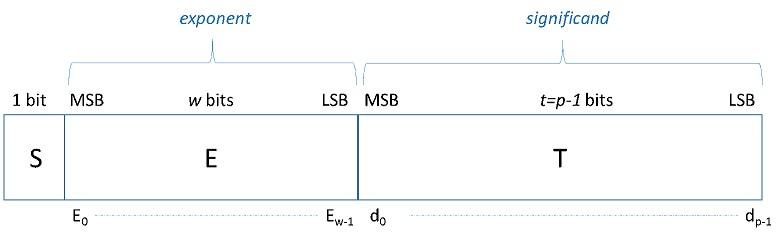
\includegraphics[scale=0.5]{format-small}
  \caption{IEEE binary format structure.}
  \label{ieee:structure}
\end{figure}

% -----------------------------------------------
\section{Representation Semantics}

\subsection{Real Values}
Most bitstreams represent a rational number, whose value v is computed using following definitions and formulas:

\begin{itemize}[topsep=0pt]
\item The bias given by $bias=emax$
\item If $1\leq E\leq 2^{w}-2$, then the number is said normal. \\
The value of the corresponding floating-point number is $v=(-1)^{S}\times 2^{{E-bias}}\times (1+2^{{1-p}}\times T)$.
\item If $E=0$ and $T\neq 0$, then the number is said denormal. \\
the value of the corresponding floating-point number is $v=(-1)^{S}\times 2^{{emin}}\times (0+2^{{1-p}}\times T)$.
\item If $E=0$ and $T=0$ , then $v=(-1)^{S}\times (+0)$.
\item If $E=2^{w}-1$ and $T=0$ , then $v=(-1)^{S}\times (+\infty )$.
\end{itemize}

\subsection{Subnormals}
According to IEEE754 standard, floating point numbers representation follows the general form $x=(-1)^S M \times 2^{exp}$ (Appendix A gives the actual correspondence between exp, M and the actual bits fields E , T).

\begin{figure}[h!]
  \centering
  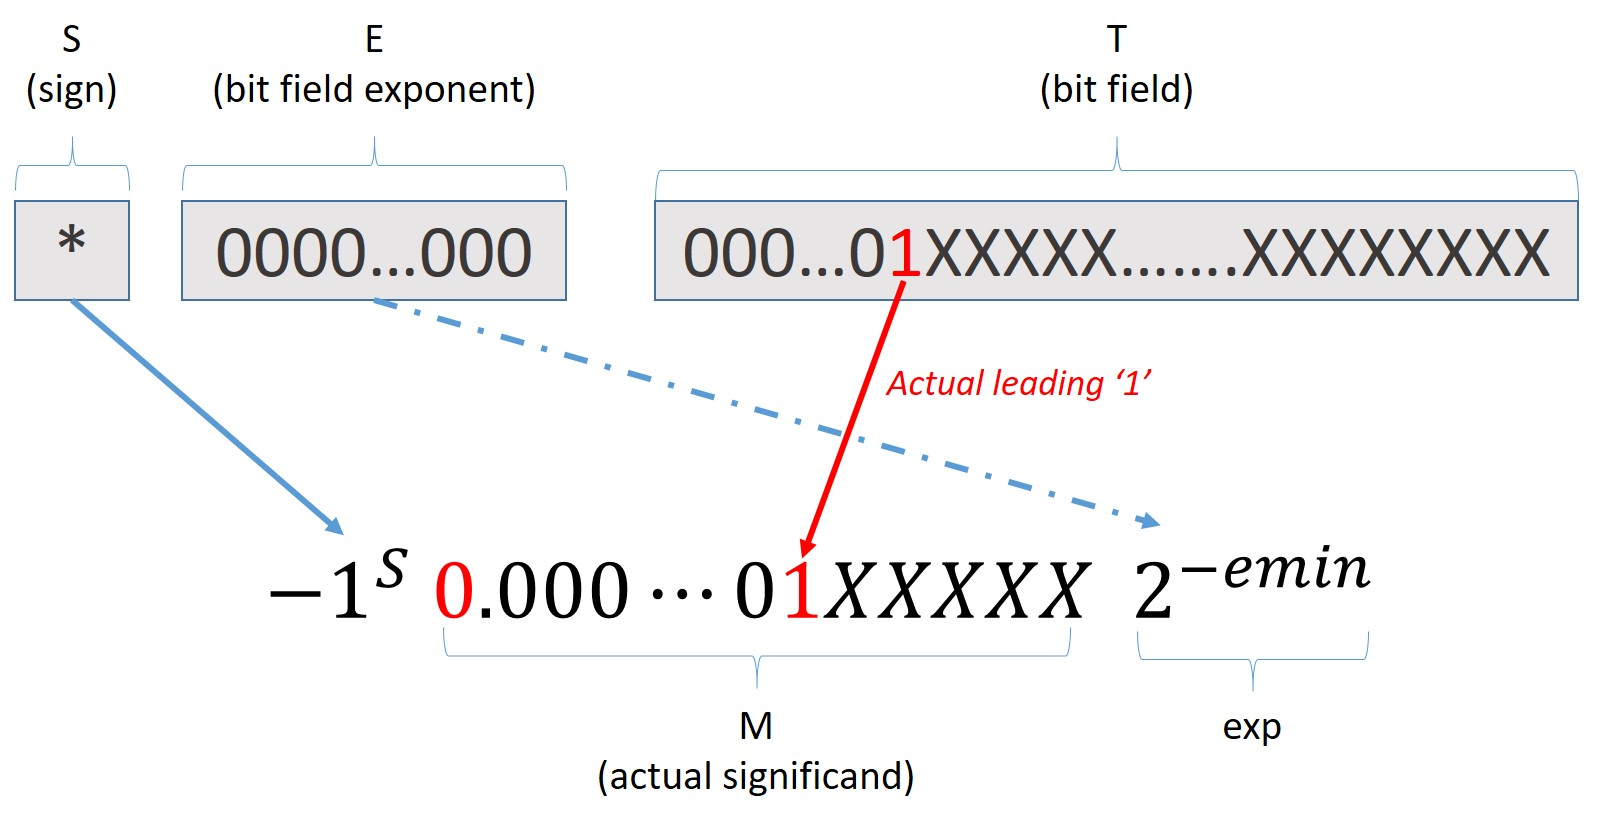
\includegraphics[scale=0.5]{subnormal}
  \caption{Subnormal representation.}
  \label{sybnormals}
\end{figure}

In the general case, we have $ 1 \leq M < 2 $ which guarantees that the representation is unique.
Since in the computer representation is finite, the exponent $exp$ can only have a finite range.  Therefore, a different rules applies for $M$ for numbers smaller than $ 1.0 \times 2^{emin}$. Those numbers are qualified as subnormals or denormals. In that case we have $ 0 < M < 1$ .

Practically, these numbers are differentiated by the encoding of field $E=0$. In that case, there is no implicit leading 1 for the mantissa:  the mantissa  stored in field T is considered with a leading 0.

\paragraph{Note:} supporting subnormals may be considered doubtful from the numerical analysis point of view, since it breaks the bound on representation relative error. However, it prevents the occurrence of underflow in subtraction. This is called gradual underflow because it allows a calculation to lose precision slowly when the result is small.

\subsection{NaNs}
\begin{itemize}[topsep=0pt]
\item If $E=2w-1$ and $T\neq 0$, the representation is a \emph{NaN} which means ``Not A Number''.
\end{itemize}
There are 2 different kinds of NaN, signaling and quiet. the most significant bit of the significand field determined whether a NaN is signaling or quiet : the value is non-zero if the NaN is quiet, and to zero if the NaN is signaling. \\
\begin{itemize}[topsep=0pt]
\item \textbf{Quiet NaNs} are used to propagate errors resulting from invalid operations or values such as overflow.
in IEEE 754, the underflow condition is only signaled if there is also a loss of precision.
\item \textbf{Signaling NaNs} can support advanced features such as mixing numerical and symbolic computation or other extensions to basic floating-point arithmetic.
\end{itemize}
% -----------------------------------------------
\section{Arithmetic Conformance}

\subsection{exactly rounded operations}
The IEEE standard requires that the result of addition, subtraction, multiplication, division, square-root, remainder, and conversion between integer and floating point formats be exactly rounded.


That is, the result must be equivalent as if computed exactly then rounded to the nearest floating-point number (using round to even). The Xvpfloat extension is only concened by exact rounding for addition, subtraction and multiplication.

\subsection{rounding rules}
The standard defines five rounding rules:
\begin{itemize}[topsep=0pt]
\item RNE: rounds to the nearest value; if the number falls midway, it is rounded to the nearest value with an even least significant digit; this is the default for binary floating point.
This corresponds to RNE rounding mode of Xvpfloat extension.
\item Round toward 0 : directed rounding towards zero (also known as truncation).
This corresponds to RTZ rounding mode of Xvpfloat extension.
\item Round toward $+\infty$  : directed rounding towards positive infinity (also known as rounding up or ceiling).
This corresponds to RUP rounding mode of Xvpfloat extension.
\item Round toward $-\infty$  : directed rounding towards negative infinity (also known as rounding down or floor).
This corresponds to RDN rounding mode of Xvpfloat extension.
\end{itemize}
These 4 modes are mandatory. The 5th rounding mode RNA is optional in radix 2, thus there is no necessity to implement it:
\begin{itemize}[topsep=0pt]
\item RNA:Round to nearest, ties away from zero : rounds to the nearest value. If the number falls midway, it is rounded to the nearest value above (for positive numbers) or below (for negative numbers).
This corresponds to RMM rounding mode of Xvpfloat extension.
\end{itemize}
At any time, one of the above four rounding modes is selected.
The programming environment should provide constants and functions for selecting (or alternatively reading) the active rounding mode dynamically in the course of a program (eg values such as \texttt{FE\_TONEAREST} or functions similar to C \emph{fesetround()}.

\paragraph{Note:} in theory, a modification of the rounding rule in a program should affect operations which appear after the change (in program order).

%% -----------------------------------------------
\section{Format configuration}

\subsection{From vpfloat language}
Within the vpfloat language, variables may be declared with constant size or dynamic size types, using the same declaration syntax, as shown in the fragment below :\\
\texttt{vpfloat<custom\_ieee, exp-info, bitsize-info> myVariable;} \\

Parameters exp-info and bit-info are integers which respectively represent the exponent and scalar bit sizes.

If exp-info and bitsize-info are not known at compile time, these parameters will be inferred at run time by a code fragment inserted at allocation time.

\paragraph{Important note:} a variable will be properly rounded to its actual significand size at store time.

\subsection{From Assembly language}
The Xvpfloat extension is only concerned about memory storage format during load and store operations.
Load and store operations will respectively decode and encode reals from/to memory according to the environment information stored in predefined registers \texttt{evp\textsubscript{i} and efp\textsubscript{i}}.
The concerned user environment is provided as an immediate in the instruction mnemonics \texttt{PLE}, \texttt{PLH}, \texttt{PLW} and \texttt{PLD} (resp \texttt{PSE}, \texttt{PSH}, \texttt{PSW} and \texttt{PSD}).

Each environment encodes following information about memory representation of variable precision numbers:
\begin{itemize}[topsep=0pt]
\item Exponent size (in bits).
\item Scalar variable footprint in memory (in bytes) is deduced from bit size rounded to the upper byte boundary.
\item Significand size (including implicit bit) is deduced from total footprint and exponent size.
\end{itemize}
There are up to 8 environments descriptors available for variable precision load/store instructions, and 8 more for half/float/double load/store instructions.
The exact behavior of load and store operations according to the environment is described in Section~\ref{sec:ls_ins}.

\chapter{Xvpfloat implementations}

\section{Rhea implementation}

\subsection{Architecture parameters}

\begin{figure}[ht]
\begin{center}
    \begin{tabular}{|l|c|p{4in}|}
    \hline
    C & 8 & Internal mantissa 64 bits chunks \\
    \hline
    ELEN & 18 & Internal exponent size (bits)\\
    \hline
    \end{tabular}
\end{center}
\caption{RISC-V Xvpfloat Rhea main parameters.}
\label{fig:Xvpfloat_rhea_main_params}
\end{figure}

\begin{figure}[ht]
\begin{center}
    \begin{tabular}{|l|c|p{4in}|}
    \hline
    MLEN & 512 & Internal mantissa size (bits) \\
    \hline
    LLEN & 3 & Internal L field size (bits)\\
    \hline
    HLEN & 26 & {\em P} register header size (bits)\\
    \hline
    VPLEN & 538 & Total size of internal scalar {\em P} register (bits)\\
    \hline
    BIS\textsubscript{MAX} & 531 & Maximum size in memory (bits)\\
    \hline
    BYS\textsubscript{MAX} & 67 & Maximum size in memory (bytes)\\
    \hline
    \end{tabular}
\end{center}
\caption{RISC-V Xvpfloat Rhea derived parameters.}
\label{fig:Xvpfloat_rhea_derived_params}
\end{figure}

\subsection{Memory formats support}

Due to issues that may happen when reading subnormal value with $ES = IEEE\_Esize_{MAX}$ (see Section~\ref{sec:subnormalFormatSupport}), we report strict and partial compliance with IEEE-754 2008 standard.
Partial compliance means that reading a subnormal number $ |x| < 2^{2^{-(ES-1)}}$ may produce incorrect results.
Xvpfloat guarantees that such a number is properly rounded when stored in memory for correct results when reading it back.

\begin{figure}[ht]
\begin{center}
    \begin{tabular}{|l|l|l|}
    \hline
                        & READ                    & WRITE \\
    \hline
                        & $2 \leq Msize \leq 512$ & $2 \leq Msize \leq 512$ \\
    \cline{2-3}
    Strict compliance   & $1 \leq Esize \leq 17$  & $1 \leq Esize \leq 18$  \\
    \cline{2-3}
                        & $1 \leq BYS \leq 66$    & $1 \leq BYS \leq 67$    \\
    \hline
                        & $2 \leq Msize \leq 512$ & $2 \leq Msize \leq 512$ \\
    \cline{2-3}
    Partial compliance  & $1 \leq Esize \leq 18$  & $1 \leq Esize \leq 18$  \\
    \cline{2-3}
                        & $1 \leq BYS \leq 67$    & $1 \leq BYS \leq 67$    \\
    \hline
    \end{tabular}
\end{center}
\caption{RISC-V Xvpfloat Rhea IEEE extendable support.}
\label{fig:Xvpfloat_rhea_ieee_extendable}
\end{figure}

\begin{figure}[ht]
\begin{center}
    \begin{tabular}{|l|l|l|l|l|l|}
    \hline
    Bitsize (k) & ES & MS  & Interchange & Strict compliance & Partial compliance \\
    \hline
    16          & 3  & 12  & X           & X                 &                    \\
    24          & 5  & 18  &             & X                 &                    \\
    32          & 7  & 24  & X           & X                 &                    \\
    40          & 8  & 31  &             & X                 &                    \\
    48          & 9  & 38  &             & X                 &                    \\
    56          & 10 & 45  &             & X                 &                    \\
    64          & 11 & 52  & X           & X                 &                    \\
    72          & 12 & 59  &             & X                 &                    \\
    80          & 12 & 67  &             & X                 &                    \\
    88          & 13 & 74  &             & X                 &                    \\
    96          & 13 & 82  &             & X                 &                    \\
    104         & 14 & 89  &             & X                 &                    \\
    112         & 14 & 97  &             & X                 &                    \\
    120         & 15 & 104 &             & X                 &                    \\
    128         & 15 & 112 & X           & X                 &                    \\
    136         & 15 & 120 &             & X                 &                    \\
    144         & 16 & 127 &             & X                 &                    \\
    152         & 16 & 135 &             & X                 &                    \\
    160         & 16 & 143 & X           & X                 &                    \\
    168         & 17 & 150 &             & X                 &                    \\
    176         & 17 & 158 &             & X                 &                    \\
    184         & 17 & 166 &             & X                 &                    \\
    192         & 17 & 174 & X           & X                 &                    \\
    200         & 18 & 181 &             &                   & X                  \\
    208         & 18 & 189 &             &                   & X                  \\
    216         & 18 & 197 &             &                   & X                  \\
    224         & 18 & 205 & X           &                   & X                  \\
    232         & 18 & 213 &             &                   & X                  \\
    \hline
    \end{tabular}
\end{center}
\caption{RISC-V Xvpfloat Rhea IEEE extended support.}
\label{fig:Xvpfloat_rhea_ieee_extended}
\end{figure}

\subsection{Performance}

\subsubsection{Forewords}

Latencies presented here are measured in isolation with an empty pipeline.
So, it does not account for back-pressure or arbitration conflicts when running other instructions in parallel.

Bandwdith reported here is measured by sending the same instruction repeatedly with the same data and parameters.

Instruction performance is both data-dependent and parameters-dependent.
As a consequence, following sections will include both models and multi-dimensionnal measurements.

\subsubsection{Addition/substraction performance}

\subsubsection{Multiplication performance}

\subsubsection{Conversion performance}

\subsubsection{Load and store performance}

\subsubsection{Move performance}

\subsubsection{Comparison performance}

\bibliographystyle{plain}
\bibliography{riscv-Xvpfloat-spec}

\end{document}
